% -*- compile-command: "make jss-slides.pdf" -*-
\documentclass{beamer}
\usepackage{tikz}
\usepackage[all]{xy}
\usepackage{amsmath,amssymb}
\usepackage{hyperref}
\usepackage{graphicx}
\usepackage{algorithmic}
\usepackage{multirow}

\DeclareMathOperator*{\argmin}{arg\,min}
\DeclareMathOperator*{\Lik}{Lik}
\DeclareMathOperator*{\PoissonLoss}{PoissonLoss}
\DeclareMathOperator*{\Peaks}{Peaks}
\DeclareMathOperator*{\Segments}{Segments}
\DeclareMathOperator*{\argmax}{arg\,max}
\DeclareMathOperator*{\maximize}{maximize}
\DeclareMathOperator*{\minimize}{minimize}
\newcommand{\sign}{\operatorname{sign}}
\newcommand{\RR}{\mathbb R}
\newcommand{\ZZ}{\mathbb Z}
\newcommand{\NN}{\mathbb N}
\newcommand{\z}{$z = 2, 4, 3, 5, 1$} 

\newcommand{\algo}[1]{\textcolor{#1}{#1}}
\definecolor{PDPA}{HTML}{66C2A5}
\definecolor{CDPA}{HTML}{FC8D62}
\definecolor{GPDPA}{HTML}{4D4D4D}

% Set transparency of non-highlighted sections in the table of
% contents slide.
\setbeamertemplate{section in toc shaded}[default][100]
\AtBeginSection[]
{
  \setbeamercolor{section in toc}{fg=red} 
  \setbeamercolor{section in toc shaded}{fg=black} 
  \begin{frame}
    \tableofcontents[currentsection]
  \end{frame}
}

\begin{document}

\title{ A Generalized Functional Pruning Optimal Partitioning (GFPOP)
  Algorithm for Peak Detection in Large Genomic Data }

\author{
  Toby Dylan Hocking\\
  toby.hocking@nau.edu\\
  joint work with \\
Guillem Rigaill, Guillaume Bourque, Paul Fearnhead}

%\date{13 Nov 2017}

\maketitle

\section{Problem: optimizing ChIP-seq peak detection}

\begin{frame}
  \frametitle{Chromatin immunoprecipitation sequencing (ChIP-seq)}
  Analysis of DNA-protein interactions.

  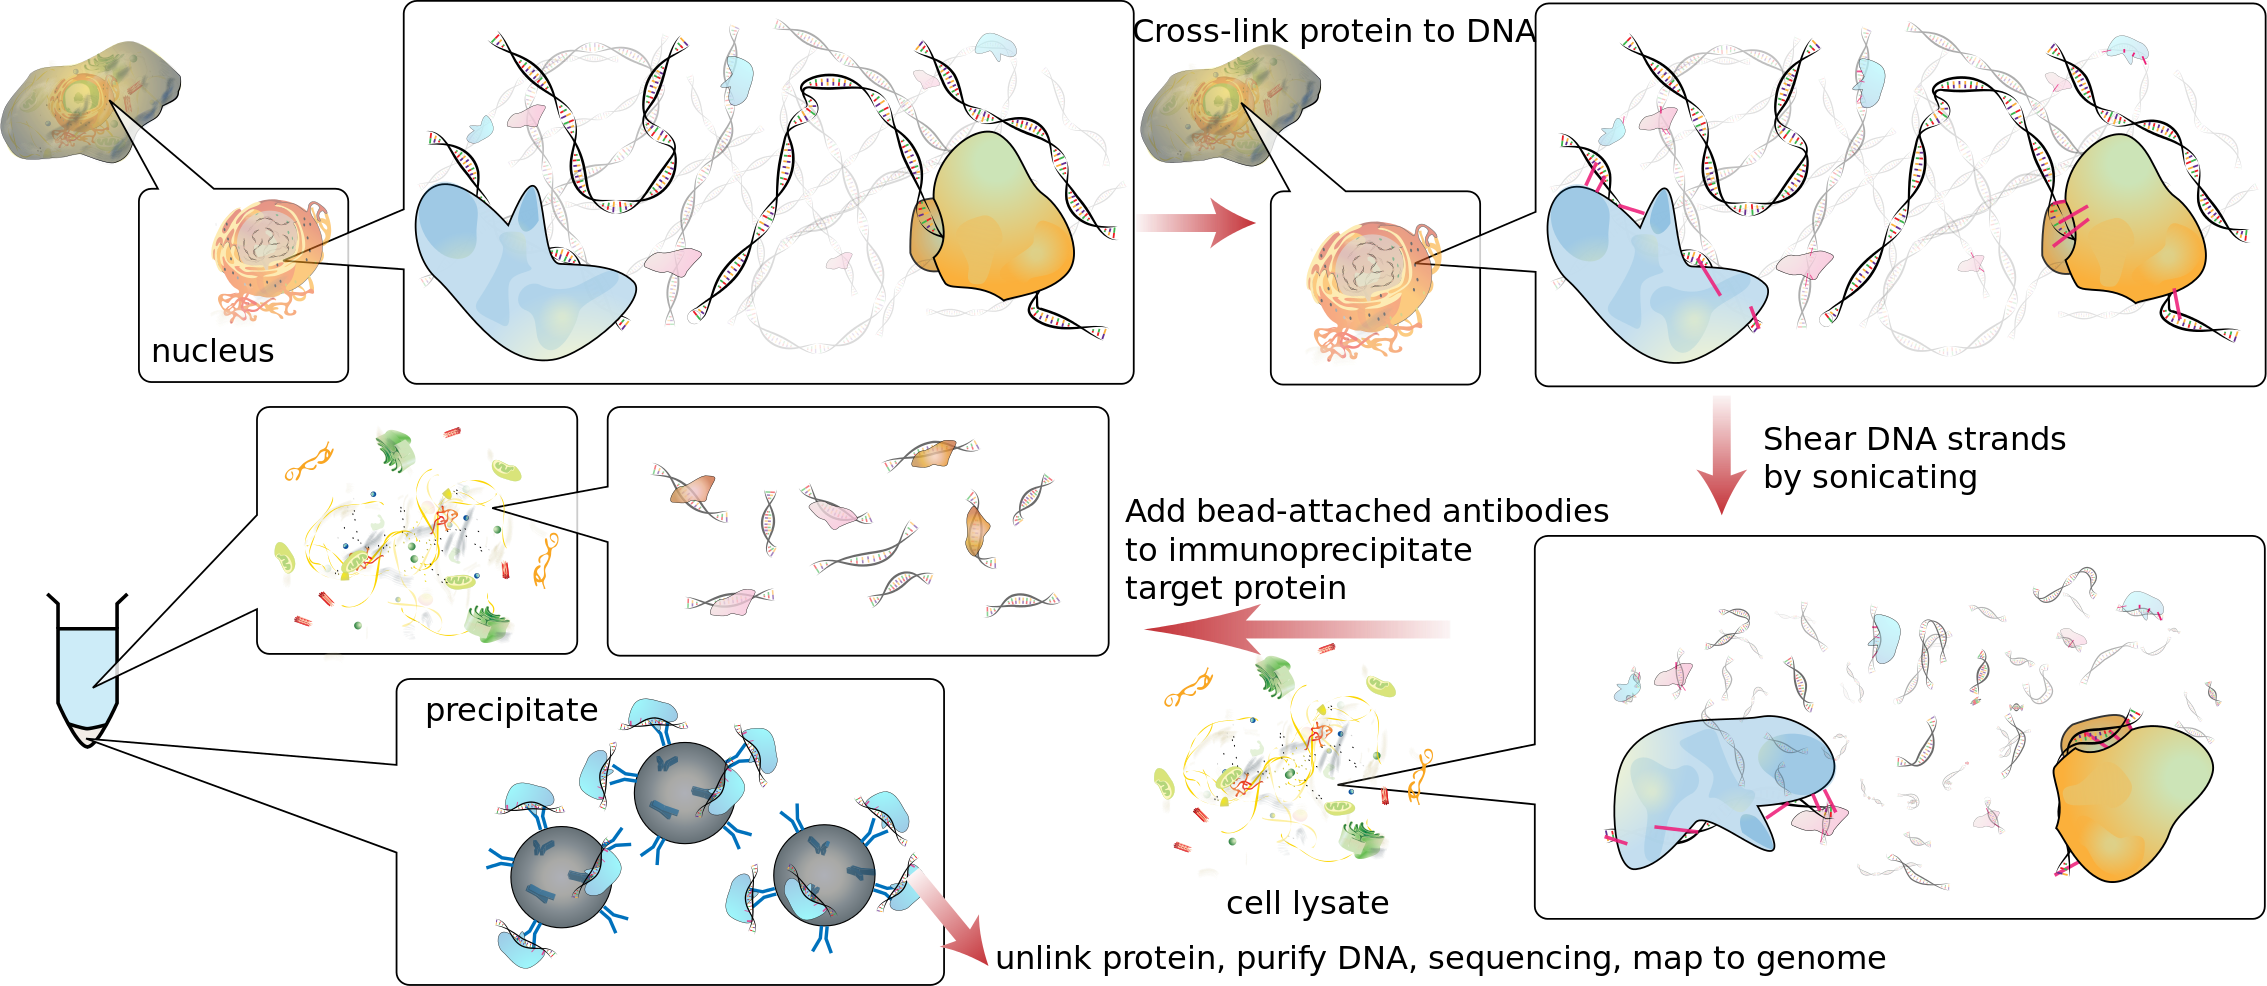
\includegraphics[width=\textwidth]{Chromatin_immunoprecipitation_sequencing_wide.png}

  Source: ``ChIP-sequencing,'' Wikipedia.
\end{frame}

\begin{frame}
  \frametitle{Problem: find peaks in each of several samples}
  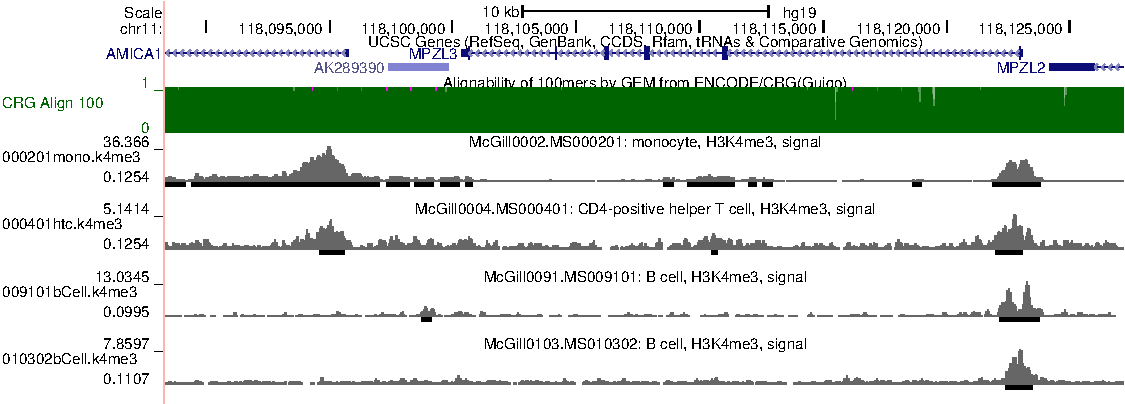
\includegraphics[width=\textwidth]{screenshot-ucsc-edited}

  \begin{itemize}
  \item Grey profiles are noisy aligned read count signals -- \\peaks
    are genomic locations with protein binding sites.
  \item Black bars are peaks called by MACS2 (Zhang et al, 2008) -- many
    false positives! (black bars where there is only noise)
  \item From a machine learning perspective, this is binary
    classification (positive=peaks, negative=noise).
  \end{itemize}
\end{frame}

% \begin{frame}
%   \frametitle{Previous work in genomic peak detection}
%   \begin{itemize}
%   \item Model-based analysis of ChIP-Seq (MACS), Zhang et al, 2008.
%   \item SICER, Zang et al, 2009.
%   \item HOMER, Heinz et al, 2010.
%   \item CCAT, Xu et al, 2010.
%   \item RSEG, Song et al, 2011.
%   \item Triform, Kornacker et al, 2012.
%   \item Histone modifications in cancer (HMCan), Ashoor et al, 2013.
%   \item PeakSeg, Hocking, Rigaill, Bourque, ICML 2015.
%   %\item PeakSegJoint Hocking and Bourque, arXiv:1506.01286.
%   \item ... dozens of others.
%   \end{itemize}
%   Two big questions: how to choose the best...
%   \begin{itemize}
%   \item ...algorithm? (testing)
%   \item \alert<1>{...parameters? (training)}
%   \end{itemize}
% \end{frame}

% \begin{frame}[fragile]
%   \frametitle{How to choose parameters of unsupervised peak
%     detectors?}
% \scriptsize
% 19 parameters for Model-based analysis of ChIP-Seq (MACS), Zhang et al, 2008.
% \begin{verbatim}
%   [-g GSIZE]
%   [-s TSIZE] [--bw BW] [-m MFOLD MFOLD] [--fix-bimodal]
%   [--nomodel] [--extsize EXTSIZE | --shiftsize SHIFTSIZE]
%   [-q QVALUE | -p PVALUE | -F FOLDENRICHMENT] [--to-large]
%   [--down-sample] [--seed SEED] [--nolambda]
%   [--slocal SMALLLOCAL] [--llocal LARGELOCAL]
%   [--shift-control] [--half-ext] [--broad]
%   [--broad-cutoff BROADCUTOFF] [--call-summits]
% \end{verbatim}
% 10 parameters for Histone modifications in cancer (HMCan),
% Ashoor et al, 2013.
% \begin{verbatim}
% minLength 145
% medLength 150
% maxLength 155
% smallBinLength 50
% largeBinLength 100000
% pvalueThreshold 0.01
% mergeDistance 200
% iterationThreshold 5
% finalThreshold 0
% maxIter 20
% \end{verbatim}
% \end{frame}
 
\begin{frame}
  \frametitle{Which macs parameter is best for these data?}
  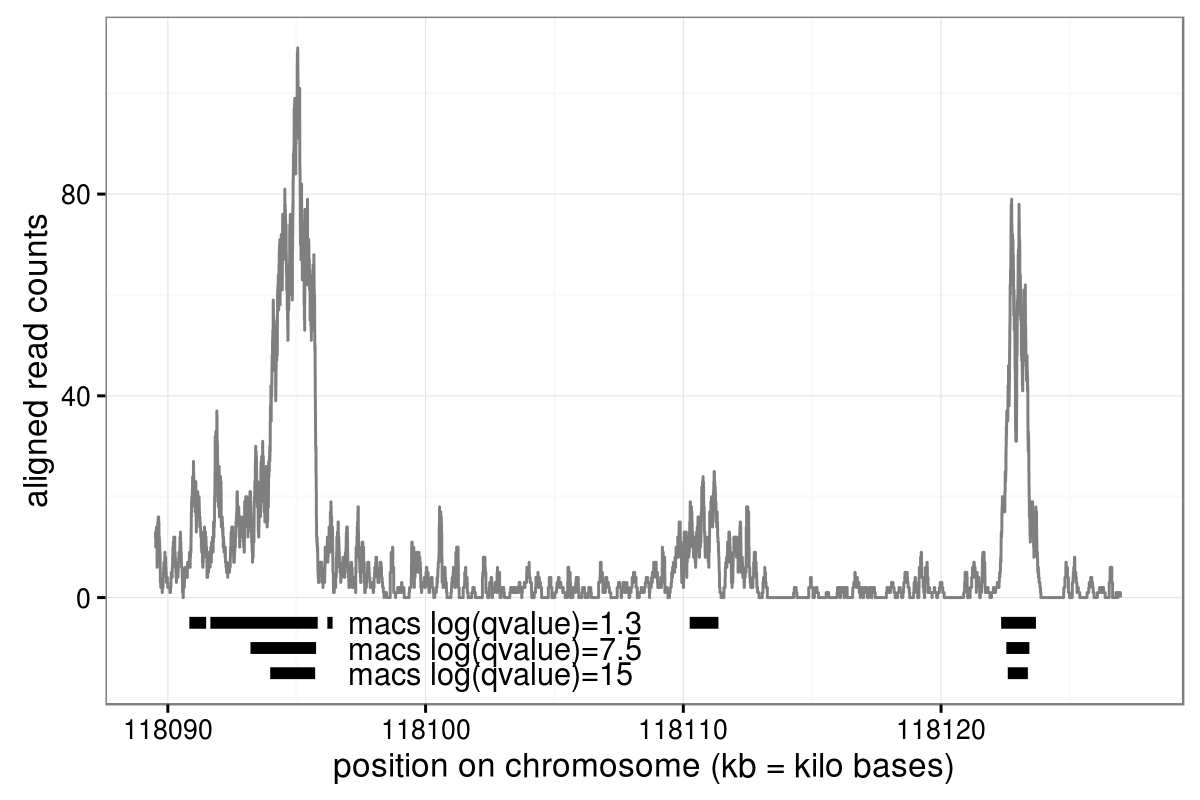
\includegraphics[width=1\textwidth]{figure-macs-problem.png}
\end{frame}

\begin{frame}
  \frametitle{Compute likelihood/loss of piecewise constant model}
  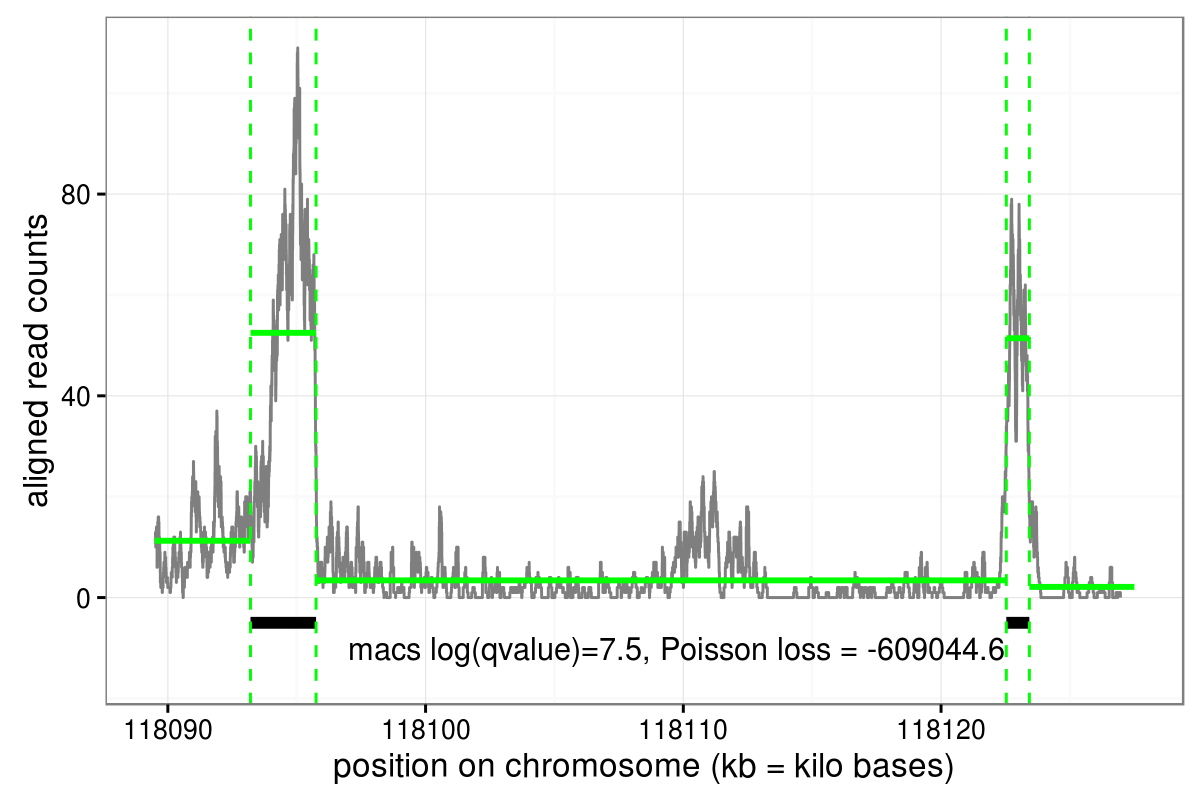
\includegraphics[width=1\textwidth]{figure-macs-problem-7-5.png}
  % $\PoissonLoss(\mathbf z, \mathbf m) = \sum_{i=1}^n m_i - z_i \log(m_i)$
  % for count data $\mathbf z\in\ZZ_+^n$ 
  % and segment mean model $\mathbf m\in\RR^n$.
\end{frame}

\begin{frame}
  \frametitle{Idea: choose the parameter with a lower loss}
  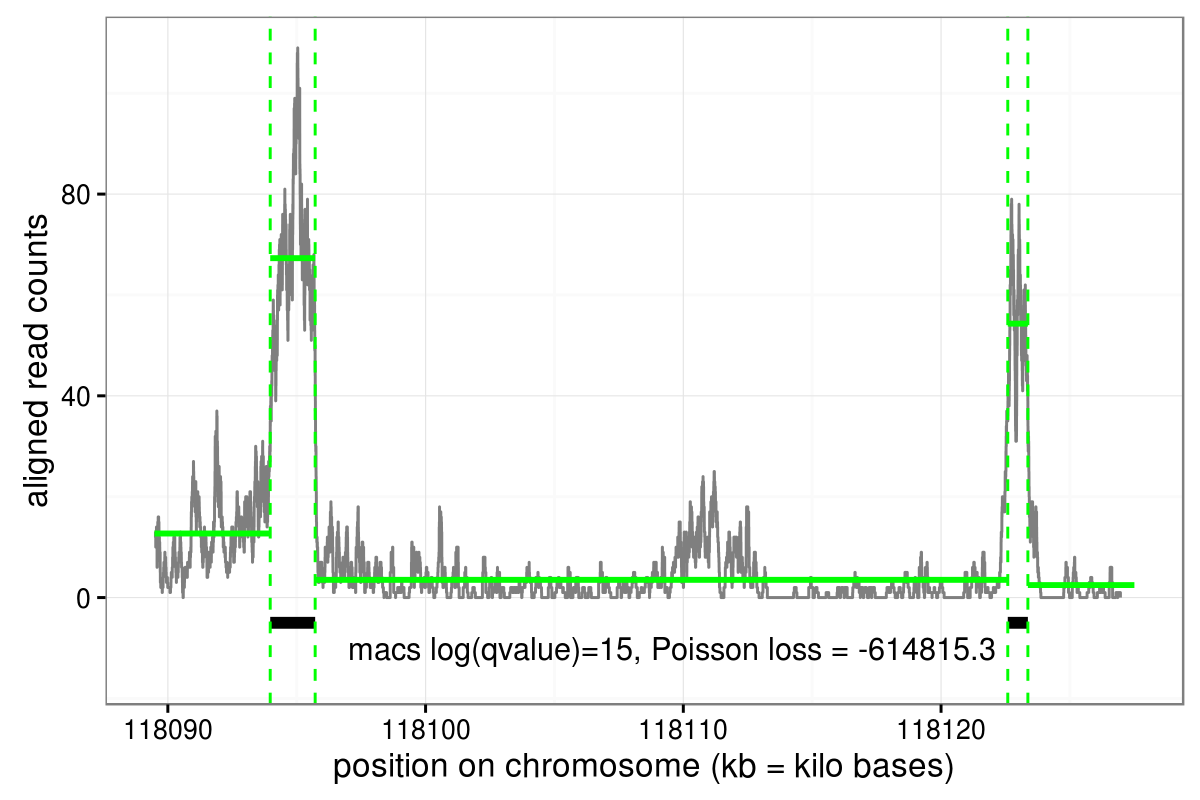
\includegraphics[width=1\textwidth]{figure-macs-problem-15.png}
\end{frame}

\begin{frame}
  \frametitle{PeakSeg: search for the peaks with lowest loss}
  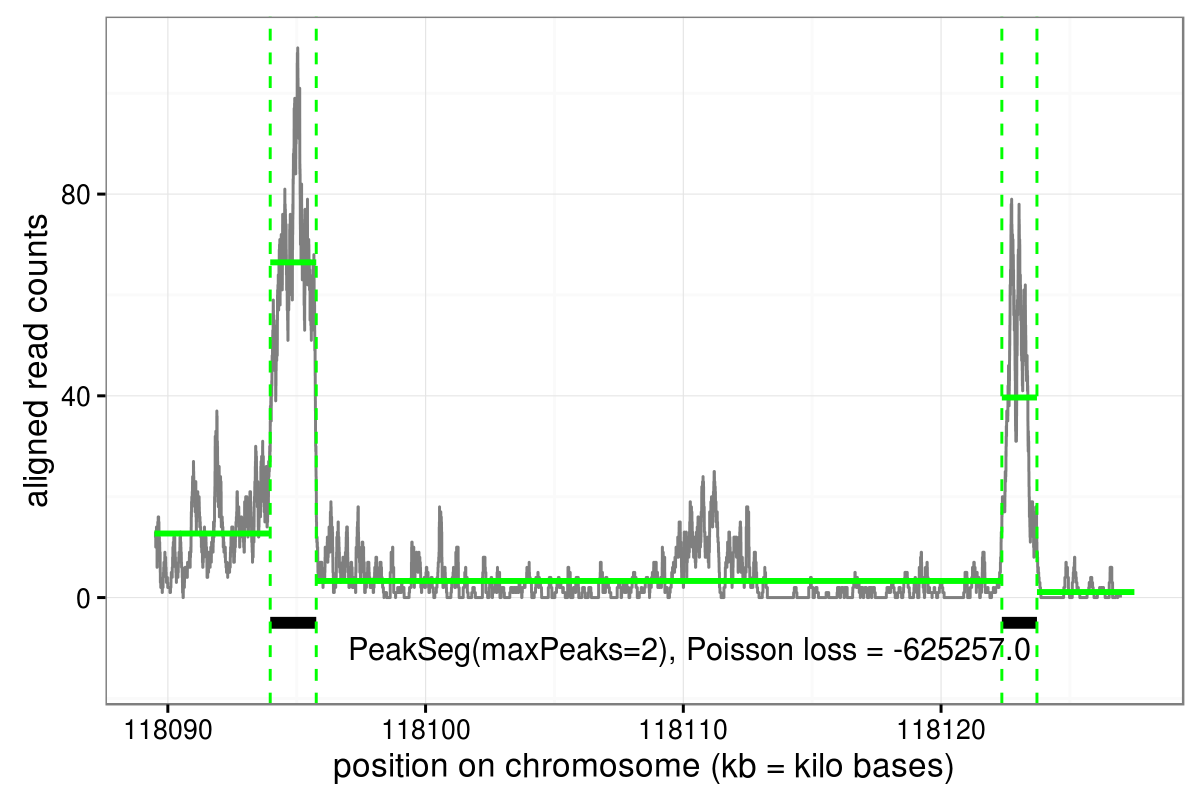
\includegraphics[width=1\textwidth]{figure-macs-problem-PeakSeg.png}

  Simple model with only one parameter (number of peaks).

  %Choose the number of peaks via standard penalties (AIC, BIC,
  %  ...)\\or learned penalties based on visual labels (more on this later).
\end{frame}

% \begin{frame}
%   \frametitle{Maximum likelihood Poisson segmentation models}
%   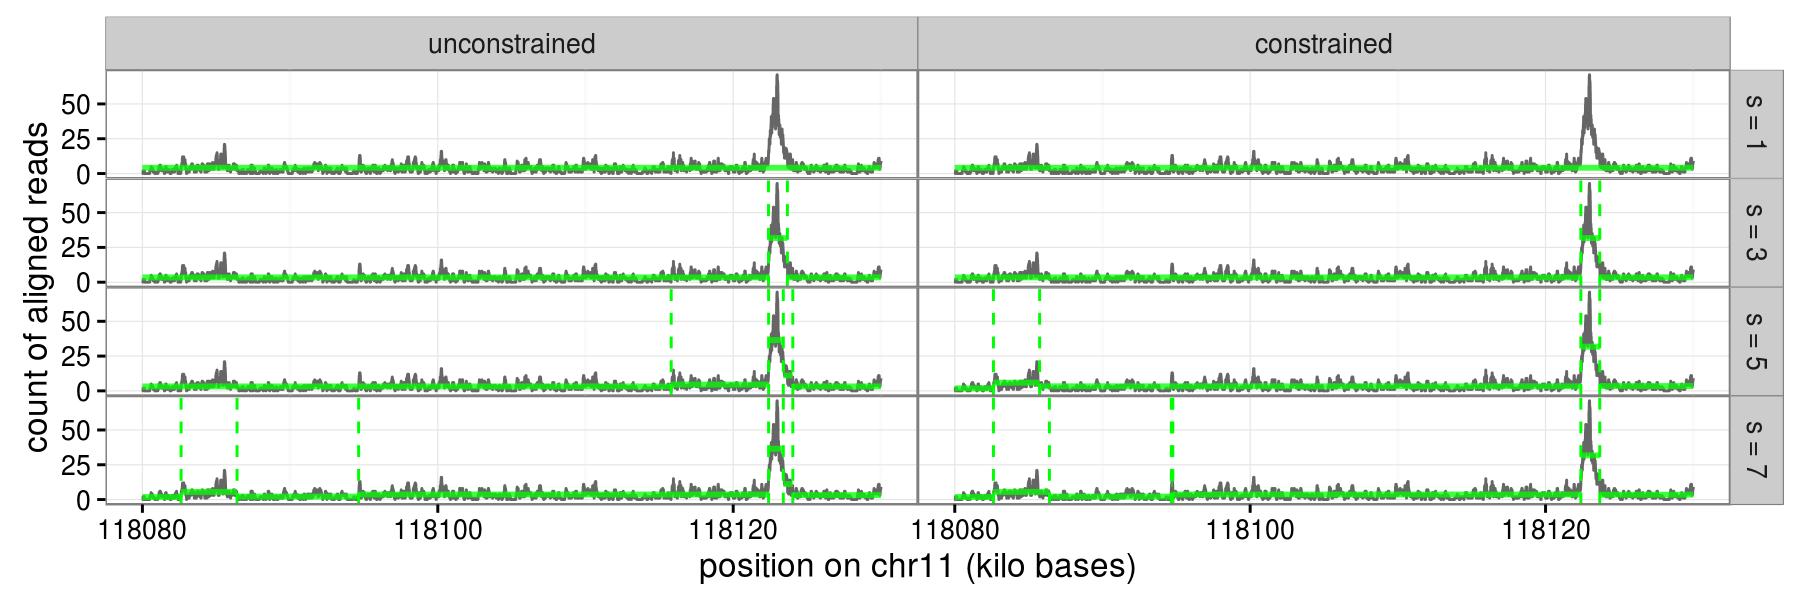
\includegraphics[width=1\textwidth]{figure-Segmentor-PeakSeg}

%   \begin{itemize}
%   \item Previous work: unconstrained maximum likelihood mean\\
%     for $s$ segments ($s-1$ changes), Cleynen et al 2014.
%   \item Hocking et al, ICML 2015: PeakSeg constraint enforces up, down, up,
%     down changes (and not up, up, down). 
%   \item Odd-numbered segments are background noise,\\
%     even-numbered segments are peaks.
%   \item Constrained Dynamic Programming Algorithm, $O(n^2)$ time for $n$ data points.
%   \end{itemize}
% \end{frame}

% \begin{frame}
%   \frametitle{But quadratic time is not fast enough for genomic data!}
%   \includegraphics[width=\textwidth]{figure-PDPA-timings-dp}
%   \begin{itemize}
%   \item Genomic data is large, $n \geq 10^6$.
%   \item Split into subsets? What if we split a peak in half?
%   \item Need linear time algorithm for analyzing whole data set.
%   \end{itemize}
% \end{frame}

\begin{frame}
  \frametitle{Statistical model is a piecewise constant Poisson mean}
  H {\it et al.}, {\it ICML} 2015. 

  \input{figure-PeakSeg}
  \vskip -0.8cm    
  \begin{itemize}
  \item We have $n$ count data $z_1, \dots, z_n\in\ZZ_+$.
  \item Fix the number of segments $S\in\{1, 2, \dots, n\}$.
  \item Optimization variables: $S-1$ changepoints
    $t_1 < \cdots < t_{S-1}$ and $S$ segment means $u_1,\dots,u_S\in\RR_+$.
  \item Let $0=t_0<t_1 < \cdots < t_{S-1}<t_S=n$ be the segment
    limits.
  \item Statistical model: for every segment $s\in\{1,\dots,S\}$,
    $z_i \stackrel{\text{iid}}{\sim} \text{Poisson}(u_s)$ for every data
    point $i\in(t_{s-1},t_s]$.
  \item PeakSeg up-down constraint: $u_1\leq u_2 \geq u_3 \leq u_4 \geq \cdots$
  \item Want to find means $u_s$ which maximize the Poisson likelihood:
    $P(Z = z_i|u_s) = u_s^{z_i} e^{-u_s} / (z_i!)$.
  \item Equivalent to finding means $u_s$ which minimize the Poisson
    loss: $\ell(u_s, z_i) = u_s - z_i\log u_s$.
  % \item Comparison to Hidden Markov Model:
  %   \begin{description}
  %   \item[Likelihood] Same emission terms, no transition terms.
  %   \item[Constraint] Number of changes rather than values.
  %   \end{description}
  \end{itemize}
\end{frame}

\begin{frame}
  \frametitle{Maximum likelihood changepoint detection with up-down constraints on adjacent segment means (PeakSeg)}
    
\only<1>{\input{figure-PeakSeg}}      
\only<2>{\input{figure-PeakSeg-unconstrained}}
\only<3>{\input{figure-PeakSeg-constrained}}
\vskip -1.4cm
\begin{align*}
    \minimize_{\substack{
  \mathbf u\in\RR^{S}
\\
   0=t_0<t_1<\cdots<t_{S-1}<t_S=N
  }} &\ \ 
    \sum_{s=1}^S\  \sum_{i=t_{s-1}+1}^{t_s} \ell( u_s,  z_i) 
\\
      \text{subject to \hskip 0.75cm} &\ \ \alert<3>{u_{s-1} \leq u_s\ \forall s\in\{2,4,\dots\},}
  \nonumber\\
  &\ \ \alert<3>{u_{s-1} \geq u_s\ \forall s\in\{3,5,\dots\}.}
  \nonumber 
\end{align*}
\vskip -0.4cm
\begin{itemize}  
\item Simple: 1 parameter = number of segments $S\in\{1,3,\dots\}$.
\item Hard optimization problem, naively $O(N^S)$ time.
\item \alert<2>{Previous unconstrained model: not always up-down changes.}
\item \alert<3>{Interpretable: $P=(S-1)/2$ peaks (segments 2, 4, ...).}
\item H {\it et al.}, {\it ICML} 2015: $O(SN^2)$ time approximate
  algorithm. 
\item H {\it et al.}, arXiv 2017: $O(SN\log N)$ time optimal algorithm.
\end{itemize}
\end{frame} 

\begin{frame}
  \frametitle{Dynamic programming with up-down constraints is highly accurate for both broad and sharp data/pattern types}
  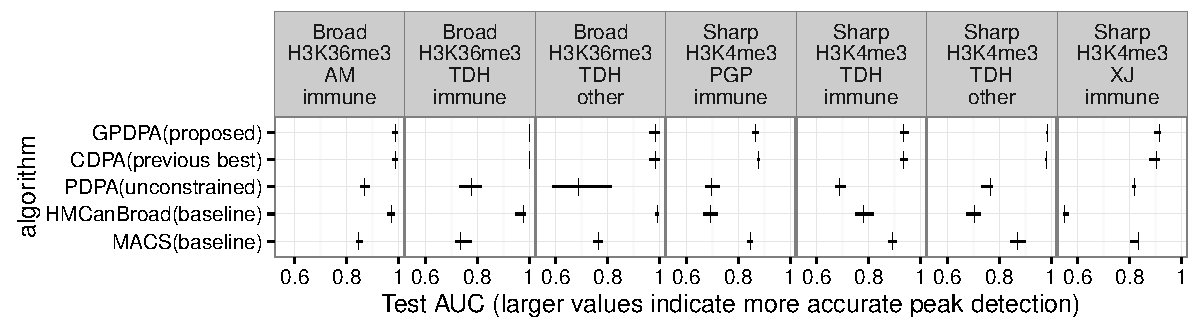
\includegraphics[width=\textwidth]{figure-test-error-dots}
  \vskip -0.5cm
  H {\it et al.}, {\it arXiv} 2017. 
  \begin{itemize}
  \item 4-fold cross-validation: train on 3/4 of labels, test on 1/4.
  \item All models trained by learning a scalar significance
    threshold / penalty parameter, which is varied to compute ROC/AUC.
  \item MACS is highly inaccurate in all data sets.
  \item HMCanBroad is accurate for broad but not sharp pattern.
  \item Unconstrained PDPA algorithm not as accurate as up-down
    constrained algorithms (CDPA, GPDPA).
  \end{itemize}
  \scriptsize
  %\url{http://bl.ocks.org/tdhock/raw/886575874144c3b172ce6b7d7d770b9f/} 
\end{frame}

\section{New functional pruning algorithm}


\begin{frame}
  \frametitle{Previous work on the Segment Neighborhood problem}
  \begin{tabular}{r|c|c}
    & no pruning & functional pruning \\
    \hline
    unconstrained & Dynamic Prog. Algo. & Pruned DPA \\
     & exact $O(SN^2)$ & exact $O(SN\log N)$\\
    %R pkgs: & \alert<1>{changepoint} & \alert<2>{cghseg, Segmentor}\\
    & Auger and L. 1989 & Rigaill 2010\\
    \hline
    up-down constrained & Constrained DPA & Generalized PDPA \\
     & inexact $O(SN^2)$ & exact $O(SN\log N)$\\
    %R pkgs: & \alert<3>{PeakSegDP} & \alert<4>{PeakSegOptimal}\\
    & H et al 2015 & H et al 2017\\
    \hline
  \end{tabular}
  \begin{itemize}
  % \item \alert<1>{Auger and Lawrence 1989, Jackson et al 2005}.
  % \item \alert<2>{Rigaill 2010, Johnson 2013, Cleynen et al 2014}.
  % \item \alert<3>{Hocking, Rigaill, Bourque 2015}.
  % \item \alert<4>{\textbf{Contribution:} Generalized Pruned Dynamic
  %       Programming Algorithm (GPDPA) that \textbf{exactly} computes the
  %     \textbf{constrained} model for $n$ data points and up to $S$ segments in
  %      $O(Sn\log n)$ time}.
  \item All algorithms solve the \textbf{Segment Neighborhood}
    ``constrained'' problem: most likely mean $m_i$ for data $z_i$,
    subject to the constraint of $S$ segments ($S-1$ changes).
  \end{itemize} 
\begin{align*}
    \minimize_{\substack{
  \mathbf m\in\RR^{N}
% \\
%    0=t_0<t_1<\cdots<t_{S-1}<t_S=N
  }} &\ \ 
    \sum_{i=1}^N \ell( m_i,  z_i) 
\\
      \text{subject to} &\ \ {\alert{\sum_{i=1}^{N-1} I[m_i\neq m_{i+1}]}=S-1,}
  \nonumber\\
  &\ \ \text{...up-down constraints on $m$.}
  \nonumber 
\end{align*}
\end{frame}

\begin{frame}
  \frametitle{Previous work on the Optimal Partitioning problem}
  \begin{tabular}{r|c|c}
    & no pruning & functional pruning \\
    \hline
    unconstrained & Opt. Part. Algo. & FPOP \\
     & exact $O(N^2)$ & exact $O(N\log N)$\\
    %R pkgs: & \alert<1>{changepoint} & \alert<2>{cghseg, Segmentor}\\
    & Jackson et al 2005 & Maidstone et al 2016\\
    \hline
    up-down constrained &  & Generalized FPOP \\
     &  & exact $O(N\log N)$\\
    %R pkgs: & \alert<3>{PeakSegDP} & \alert<4>{PeakSegOptimal}\\
    &  & \textbf{This work}\\
    \hline
  \end{tabular}
  \begin{itemize}
  % \item \alert<1>{Auger and Lawrence 1989, Jackson et al 2005}.
  % \item \alert<2>{Rigaill 2010, Johnson 2013, Cleynen et al 2014}.
  % \item \alert<3>{Hocking, Rigaill, Bourque 2015}.
  % \item \alert<4>{\textbf{Contribution:} Generalized Pruned Dynamic
  %       Programming Algorithm (GPDPA) that \textbf{exactly} computes the
  %     \textbf{constrained} model for $n$ data points and up to $S$ segments in
  %      $O(Sn\log n)$ time}.
  \item All algorithms solve the \textbf{Optimal Partitioning}
    ``penalized'' problem: most likely mean $m_i$ for data $z_i$,
    penalized by a non-negative penalty $\lambda\in\RR_+$ for each change:
  \end{itemize}
\begin{align*}
    \minimize_{\substack{
  \mathbf m\in\RR^{N}
% \\
%    0=t_0<t_1<\cdots<t_{S-1}<t_S=N
  }} &\ \ 
    \sum_{i=1}^N \ell( m_i,  z_i)  + \lambda\alert{\sum_{i=1}^{N-1}I[m_{i}\neq m_{i+1}]}
\\
      \text{subject to} &\ \ \text{...up-down constraints on $m$.}
  \nonumber 
\end{align*}
\end{frame}


\begin{frame}
  \frametitle{Dynamic programming and functional pruning}
  \textbf{Classical dynamic programming for optimal partitioning}
  (Jackson et al 2005) computes the vector of optimal loss values up
  to $N$ data points, $O(N^2)$ time because each DP iteration needs to
  consider all $O(N)$ possible changepoints and cost values.
$$
\begin{array}{ccccc}
  \mathcal C_{1} & \mathcal C_2 & \cdots & \mathcal C_{N-1} &  \mathcal C_N
\end{array}
$$
\textbf{Functional pruning optimal partitioning} (Maidstone 2016)
computes a vector of loss \textbf{functions}, $O(N\log N)$ because
each DP iteration only considers $O(\log N)$ candidate changepoints
\\(the others --- which will never be optimal --- are pruned).
$$
\begin{array}{ccccc}
   C_{1}(m_1) & C_2(m_2) & \cdots & C_{N-1}(m_{N-1}) &   C_N(m_{N})
\end{array}
$$
\textbf{Contribution of this work}: a new algorithm that applies the
functional pruning technique to the up-down constrained model.
\end{frame}

\begin{frame}
  \frametitle{Constrained optimal partitioning problem}
  \begin{align*}
  \label{eq:penalized_peakseg}
  \minimize_{
    \substack{
    \mathbf m\in\RR^N,\ \mathbf s\in\{0, 1\}^N\\
\mathbf c\in\{-1, 0,1\}^{N-1}\\
}
    } &\ \ 
  \sum_{i=1}^N \ell(m_i, z_i) + \lambda \sum_{i=1}^{N-1} I(c_i \neq 0) \\
  \text{subject to\ \ } &\ \text{no change: }c_t = 0 \Rightarrow m_t = m_{t+1}\text{ and }s_t=s_{t+1}
  \nonumber\\
&\ \text{go up: }c_t = 1 \Rightarrow m_t \leq m_{t+1}\text{ and }(s_t,s_{t+1})=(0,1),
  \nonumber\\
&\ \text{go down: } c_t = -1 \Rightarrow m_t \geq m_{t+1}\text{ and }(s_t,s_{t+1})=(1,0).
\nonumber
\end{align*}
\begin{minipage}{0.5\linewidth}
    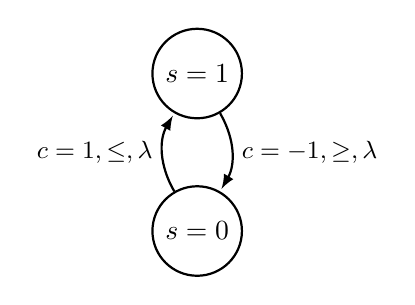
\begin{tikzpicture}[->,>=latex,shorten >=1pt,auto,node distance=2cm,
                    thick,main node/.style={circle,draw}]

  \node[main node] (1) {$s=1$};
  \node[main node] (2) [below of=1] {$s=0$};

  \path[every node/.style={font=\sffamily\small}]
    (2) edge [bend left] node {$c=1, \leq, \lambda$} (1)
    (1) edge [bend left] node {$c=-1, \geq, \lambda$} (2);
\end{tikzpicture}
\end{minipage}
\begin{minipage}{0.45\linewidth}
  Nodes=states $s$,\\
  Edges=changes $c$ (constraint, penalty).
\end{minipage}
\end{frame}

\begin{frame}
  \frametitle{Generalized Functional Pruning Optimal Partitioning
    (GFPOP) algorithm for up-down constrained model}
Recursively compute two vectors of real-valued cost functions:
$$
\begin{array}{cccl}
  \overline C_{1}(m_1) & \cdots & \overline C_N(m_{N})& \text{ optimal cost in peak state $s=1$}\\
  \underline C_{1}(m_1) & \cdots & \underline C_N(m_{N})& \text{ optimal cost in background state $s=0$}\\
\end{array}
$$
\begin{minipage}{0.65\linewidth}
  $$\overline C_{t+1}(\mu) = \ell(\mu, z_i) + \min\{
  \overline C_t(\mu),\, 
  \underline C_t^\leq(\mu)+\lambda
\},$$
  $$\underline C_{t+1}(\mu) = \ell(\mu, z_i) + \min\{
  \underline C_t(\mu),\, 
  \overline C_t^\geq(\mu)+\lambda
\},$$
where $f^\leq(\mu) = \min_{x\leq\mu} f(x)$,\\
$f^\geq(\mu) = \min_{x\geq\mu} f(x)$.
\end{minipage}
\begin{minipage}{0.25\linewidth}
  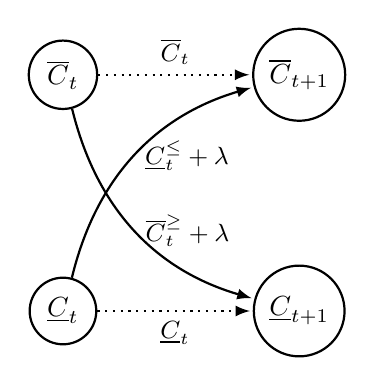
\begin{tikzpicture}[->,>=latex,shorten >=1pt,auto,node distance=3cm,
  thick,main node/.style={circle,draw}]
  \node[main node] (peak_t) {$\overline C_t$};
  \node[main node] (bkg_t) [below of=peak_t] {$\underline C_t$};
  \node[main node] (peak_t1) [right of=peak_t] {$\overline C_{t+1}$};
  \node[main node] (bkg_t1) [right of=bkg_t] {$\underline C_{t+1}$};
  \path[every node/.style={font=\small}]
    (peak_t) edge [dotted] node {$\overline C_{t}$} (peak_t1)
    (peak_t) edge [black, bend right] node [right] {$\overline C_{t}^{\geq}+\lambda$} (bkg_t1)
    (bkg_t) edge [dotted] node[midway, below] {$\underline C_{t}$} (bkg_t1)
    (bkg_t) edge [black, bend left] node[right] {$\underline C_{ t}^{\leq}+\lambda$} (peak_t1)
;
\end{tikzpicture}
\end{minipage}
\end{frame}

\section{Results on ChIP-seq benchmark}

\begin{frame}
  \frametitle{Benchmark of large genomic data sequences}

\url{http://github.com/tdhock/feature-learning-benchmark}

\begin{itemize}
\item 4951 data sequences ranging from $N=10^3$ to $N=10^7$.
\item Ran GFPOP with penalty $\lambda\in(\log N, N)$, resulting in a
  range of models with different numbers of peaks, for each data set.
\item Each data set has \textbf{labels} which can be used to determine
  an appropriate number of peaks.
\end{itemize}
\end{frame}

\begin{frame}
  \frametitle{Labels used to determine optimal number of peaks}
  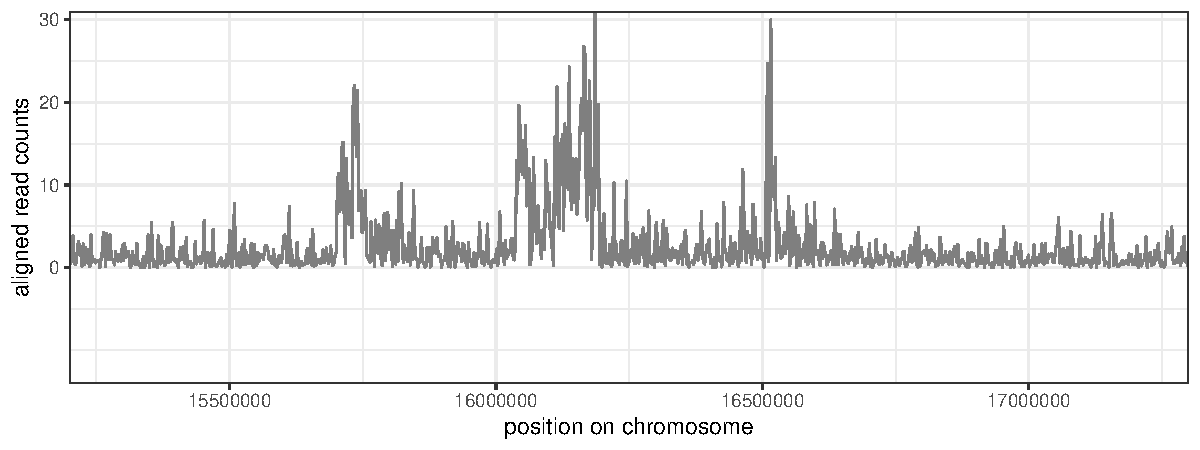
\includegraphics[width=\textwidth]{jss-figure-label-error-data}
  
  One ChIP-seq data set with $N=1,254,751$ (only 82,233 shown).
\end{frame}

\begin{frame}
  \frametitle{Labels used to determine optimal number of peaks}
  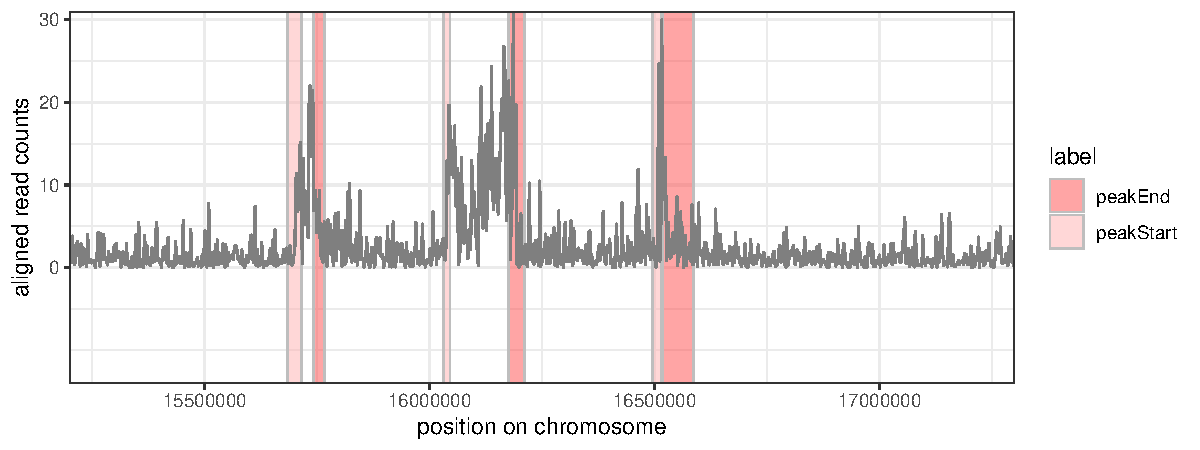
\includegraphics[width=\textwidth]{jss-figure-label-error-data-labels}

  Visually labeled regions (H {\it et al.}, {\it Bioinformatics} 2017). 
\end{frame}

\begin{frame}
  \frametitle{Labels used to determine optimal number of peaks}
  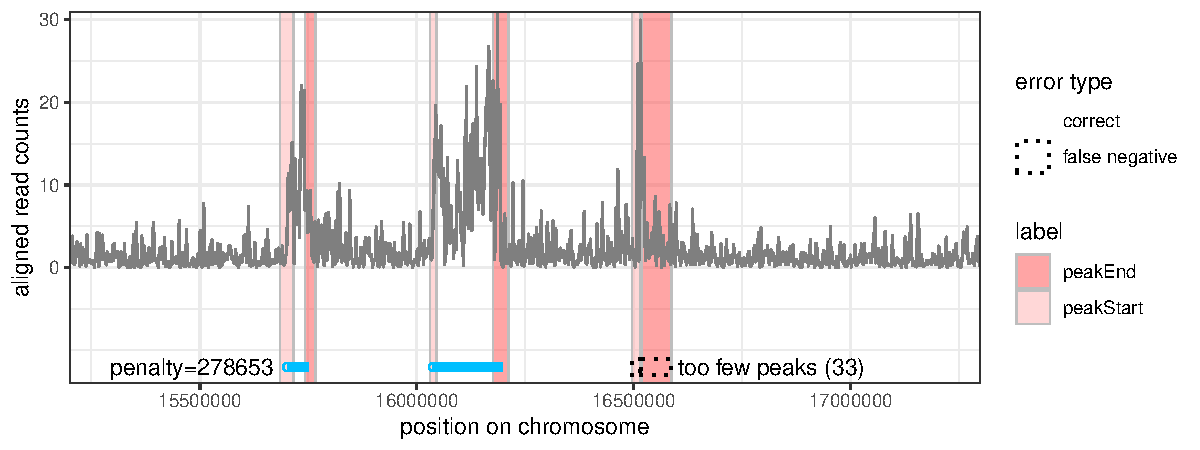
\includegraphics[width=\textwidth]{jss-figure-label-error-too-few}

  Penalty too large, too few peaks, 2 false negative labels.
\end{frame}

\begin{frame}
  \frametitle{Labels used to determine optimal number of peaks}
  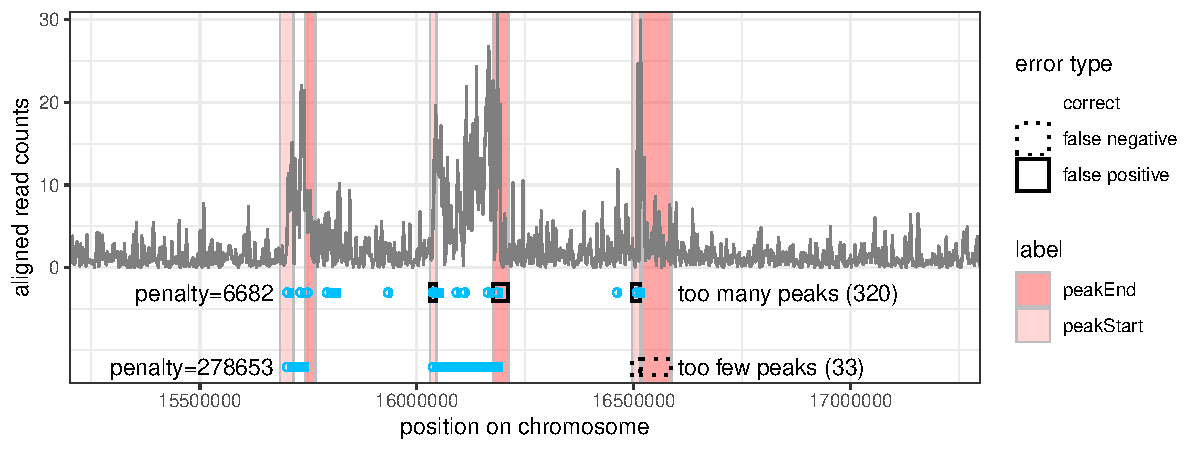
\includegraphics[width=\textwidth]{jss-figure-label-error-too-many}

  Penalty too small, too many peaks, 3 false positive labels.
\end{frame}

\begin{frame}
  \frametitle{Labels used to determine optimal number of peaks}
  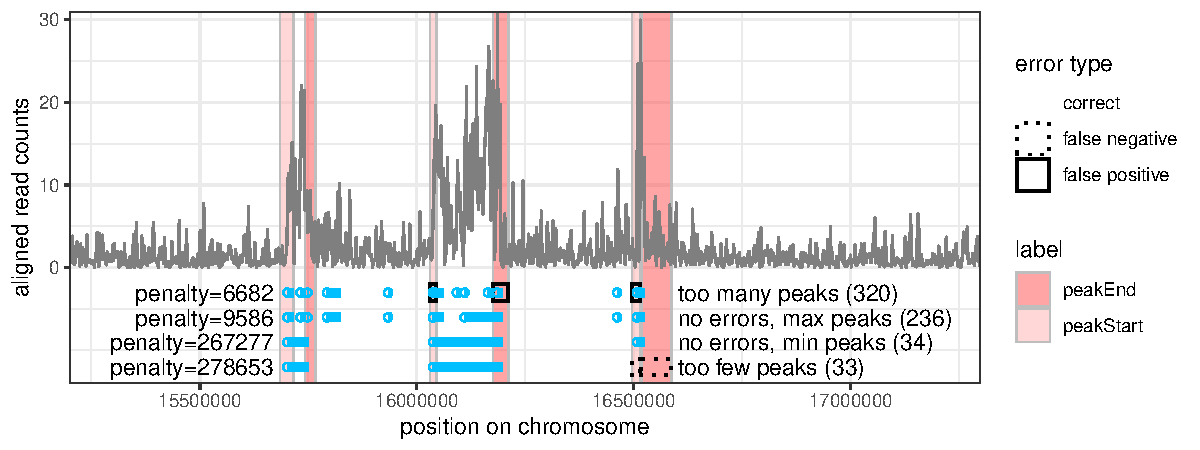
\includegraphics[width=\textwidth]{jss-figure-label-error}
  
  Models with 34--236 peaks have no label errors (midpoint=135).
\end{frame}

\begin{frame}
  \frametitle{Segment Neighborhood model too slow for $O(\sqrt N)$ peaks }
  % Created by tikzDevice version 0.12.3.1 on 2021-08-27 10:42:22
% !TEX encoding = UTF-8 Unicode
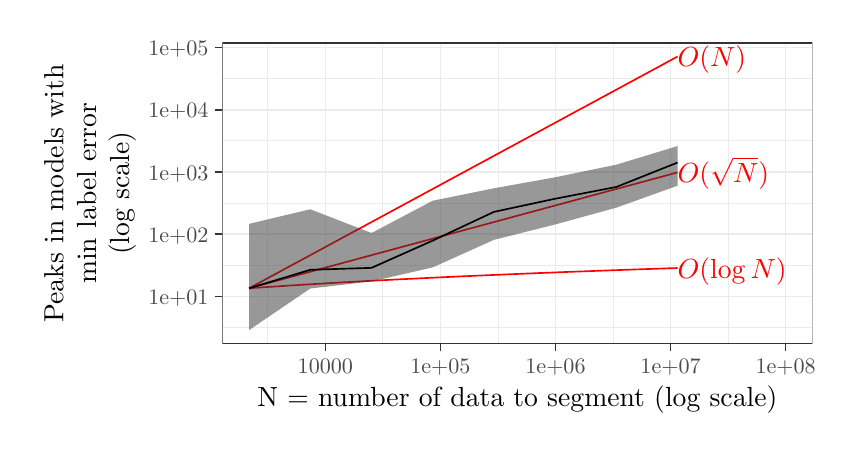
\begin{tikzpicture}[x=1pt,y=1pt]
\definecolor{fillColor}{RGB}{255,255,255}
\path[use as bounding box,fill=fillColor,fill opacity=0.00] (0,0) rectangle (289.08,144.54);
\begin{scope}
\path[clip] (  0.00,  0.00) rectangle (289.08,144.54);
\definecolor{drawColor}{RGB}{255,255,255}
\definecolor{fillColor}{RGB}{255,255,255}

\path[draw=drawColor,line width= 0.6pt,line join=round,line cap=round,fill=fillColor] (  0.00,  0.00) rectangle (289.08,144.54);
\end{scope}
\begin{scope}
\path[clip] ( 70.31, 30.33) rectangle (283.58,139.04);
\definecolor{fillColor}{RGB}{255,255,255}

\path[fill=fillColor] ( 70.31, 30.33) rectangle (283.58,139.04);
\definecolor{drawColor}{gray}{0.92}

\path[draw=drawColor,line width= 0.3pt,line join=round] ( 70.31, 36.20) --
	(283.58, 36.20);

\path[draw=drawColor,line width= 0.3pt,line join=round] ( 70.31, 58.68) --
	(283.58, 58.68);

\path[draw=drawColor,line width= 0.3pt,line join=round] ( 70.31, 81.17) --
	(283.58, 81.17);

\path[draw=drawColor,line width= 0.3pt,line join=round] ( 70.31,103.65) --
	(283.58,103.65);

\path[draw=drawColor,line width= 0.3pt,line join=round] ( 70.31,126.14) --
	(283.58,126.14);

\path[draw=drawColor,line width= 0.3pt,line join=round] ( 86.78, 30.33) --
	( 86.78,139.04);

\path[draw=drawColor,line width= 0.3pt,line join=round] (128.36, 30.33) --
	(128.36,139.04);

\path[draw=drawColor,line width= 0.3pt,line join=round] (169.94, 30.33) --
	(169.94,139.04);

\path[draw=drawColor,line width= 0.3pt,line join=round] (211.52, 30.33) --
	(211.52,139.04);

\path[draw=drawColor,line width= 0.3pt,line join=round] (253.10, 30.33) --
	(253.10,139.04);

\path[draw=drawColor,line width= 0.6pt,line join=round] ( 70.31, 47.44) --
	(283.58, 47.44);

\path[draw=drawColor,line width= 0.6pt,line join=round] ( 70.31, 69.93) --
	(283.58, 69.93);

\path[draw=drawColor,line width= 0.6pt,line join=round] ( 70.31, 92.41) --
	(283.58, 92.41);

\path[draw=drawColor,line width= 0.6pt,line join=round] ( 70.31,114.90) --
	(283.58,114.90);

\path[draw=drawColor,line width= 0.6pt,line join=round] ( 70.31,137.38) --
	(283.58,137.38);

\path[draw=drawColor,line width= 0.6pt,line join=round] (107.57, 30.33) --
	(107.57,139.04);

\path[draw=drawColor,line width= 0.6pt,line join=round] (149.15, 30.33) --
	(149.15,139.04);

\path[draw=drawColor,line width= 0.6pt,line join=round] (190.73, 30.33) --
	(190.73,139.04);

\path[draw=drawColor,line width= 0.6pt,line join=round] (232.31, 30.33) --
	(232.31,139.04);

\path[draw=drawColor,line width= 0.6pt,line join=round] (273.89, 30.33) --
	(273.89,139.04);
\definecolor{drawColor}{RGB}{255,0,0}

\path[draw=drawColor,line width= 0.6pt,line join=round] ( 80.01, 50.37) --
	( 81.57, 50.48) --
	( 83.13, 50.59) --
	( 84.70, 50.70) --
	( 86.26, 50.80) --
	( 87.82, 50.91) --
	( 89.39, 51.01) --
	( 90.95, 51.11) --
	( 92.52, 51.22) --
	( 94.08, 51.32) --
	( 95.64, 51.42) --
	( 97.21, 51.51) --
	( 98.77, 51.61) --
	(100.34, 51.71) --
	(101.90, 51.80) --
	(103.46, 51.90) --
	(105.03, 51.99) --
	(106.59, 52.08) --
	(108.16, 52.18) --
	(109.72, 52.27) --
	(111.28, 52.36) --
	(112.85, 52.45) --
	(114.41, 52.54) --
	(115.97, 52.62) --
	(117.54, 52.71) --
	(119.10, 52.80) --
	(120.67, 52.88) --
	(122.23, 52.97) --
	(123.79, 53.05) --
	(125.36, 53.13) --
	(126.92, 53.22) --
	(128.49, 53.30) --
	(130.05, 53.38) --
	(131.61, 53.46) --
	(133.18, 53.54) --
	(134.74, 53.62) --
	(136.31, 53.70) --
	(137.87, 53.78) --
	(139.43, 53.85) --
	(141.00, 53.93) --
	(142.56, 54.01) --
	(144.12, 54.08) --
	(145.69, 54.16) --
	(147.25, 54.23) --
	(148.82, 54.31) --
	(150.38, 54.38) --
	(151.94, 54.45) --
	(153.51, 54.52) --
	(155.07, 54.60) --
	(156.64, 54.67) --
	(158.20, 54.74) --
	(159.76, 54.81) --
	(161.33, 54.88) --
	(162.89, 54.95) --
	(164.46, 55.01) --
	(166.02, 55.08) --
	(167.58, 55.15) --
	(169.15, 55.22) --
	(170.71, 55.28) --
	(172.27, 55.35) --
	(173.84, 55.42) --
	(175.40, 55.48) --
	(176.97, 55.55) --
	(178.53, 55.61) --
	(180.09, 55.68) --
	(181.66, 55.74) --
	(183.22, 55.80) --
	(184.79, 55.87) --
	(186.35, 55.93) --
	(187.91, 55.99) --
	(189.48, 56.05) --
	(191.04, 56.11) --
	(192.61, 56.17) --
	(194.17, 56.24) --
	(195.73, 56.30) --
	(197.30, 56.36) --
	(198.86, 56.41) --
	(200.42, 56.47) --
	(201.99, 56.53) --
	(203.55, 56.59) --
	(205.12, 56.65) --
	(206.68, 56.71) --
	(208.24, 56.76) --
	(209.81, 56.82) --
	(211.37, 56.88) --
	(212.94, 56.93) --
	(214.50, 56.99) --
	(216.06, 57.05) --
	(217.63, 57.10) --
	(219.19, 57.16) --
	(220.76, 57.21) --
	(222.32, 57.27) --
	(223.88, 57.32) --
	(225.45, 57.37) --
	(227.01, 57.43) --
	(228.58, 57.48) --
	(230.14, 57.53) --
	(231.70, 57.59) --
	(233.27, 57.64) --
	(234.83, 57.69);

\path[draw=drawColor,line width= 0.6pt,line join=round] ( 80.01, 50.37) --
	( 81.57, 50.80) --
	( 83.13, 51.22) --
	( 84.70, 51.64) --
	( 86.26, 52.06) --
	( 87.82, 52.49) --
	( 89.39, 52.91) --
	( 90.95, 53.33) --
	( 92.52, 53.76) --
	( 94.08, 54.18) --
	( 95.64, 54.60) --
	( 97.21, 55.02) --
	( 98.77, 55.45) --
	(100.34, 55.87) --
	(101.90, 56.29) --
	(103.46, 56.72) --
	(105.03, 57.14) --
	(106.59, 57.56) --
	(108.16, 57.98) --
	(109.72, 58.41) --
	(111.28, 58.83) --
	(112.85, 59.25) --
	(114.41, 59.68) --
	(115.97, 60.10) --
	(117.54, 60.52) --
	(119.10, 60.94) --
	(120.67, 61.37) --
	(122.23, 61.79) --
	(123.79, 62.21) --
	(125.36, 62.64) --
	(126.92, 63.06) --
	(128.49, 63.48) --
	(130.05, 63.90) --
	(131.61, 64.33) --
	(133.18, 64.75) --
	(134.74, 65.17) --
	(136.31, 65.60) --
	(137.87, 66.02) --
	(139.43, 66.44) --
	(141.00, 66.86) --
	(142.56, 67.29) --
	(144.12, 67.71) --
	(145.69, 68.13) --
	(147.25, 68.56) --
	(148.82, 68.98) --
	(150.38, 69.40) --
	(151.94, 69.82) --
	(153.51, 70.25) --
	(155.07, 70.67) --
	(156.64, 71.09) --
	(158.20, 71.52) --
	(159.76, 71.94) --
	(161.33, 72.36) --
	(162.89, 72.78) --
	(164.46, 73.21) --
	(166.02, 73.63) --
	(167.58, 74.05) --
	(169.15, 74.48) --
	(170.71, 74.90) --
	(172.27, 75.32) --
	(173.84, 75.74) --
	(175.40, 76.17) --
	(176.97, 76.59) --
	(178.53, 77.01) --
	(180.09, 77.44) --
	(181.66, 77.86) --
	(183.22, 78.28) --
	(184.79, 78.70) --
	(186.35, 79.13) --
	(187.91, 79.55) --
	(189.48, 79.97) --
	(191.04, 80.40) --
	(192.61, 80.82) --
	(194.17, 81.24) --
	(195.73, 81.66) --
	(197.30, 82.09) --
	(198.86, 82.51) --
	(200.42, 82.93) --
	(201.99, 83.36) --
	(203.55, 83.78) --
	(205.12, 84.20) --
	(206.68, 84.62) --
	(208.24, 85.05) --
	(209.81, 85.47) --
	(211.37, 85.89) --
	(212.94, 86.32) --
	(214.50, 86.74) --
	(216.06, 87.16) --
	(217.63, 87.58) --
	(219.19, 88.01) --
	(220.76, 88.43) --
	(222.32, 88.85) --
	(223.88, 89.28) --
	(225.45, 89.70) --
	(227.01, 90.12) --
	(228.58, 90.54) --
	(230.14, 90.97) --
	(231.70, 91.39) --
	(233.27, 91.81) --
	(234.83, 92.24);

\path[draw=drawColor,line width= 0.6pt,line join=round] ( 80.01, 50.37) --
	( 81.57, 51.22) --
	( 83.13, 52.06) --
	( 84.70, 52.91) --
	( 86.26, 53.76) --
	( 87.82, 54.60) --
	( 89.39, 55.45) --
	( 90.95, 56.29) --
	( 92.52, 57.14) --
	( 94.08, 57.98) --
	( 95.64, 58.83) --
	( 97.21, 59.68) --
	( 98.77, 60.52) --
	(100.34, 61.37) --
	(101.90, 62.21) --
	(103.46, 63.06) --
	(105.03, 63.90) --
	(106.59, 64.75) --
	(108.16, 65.60) --
	(109.72, 66.44) --
	(111.28, 67.29) --
	(112.85, 68.13) --
	(114.41, 68.98) --
	(115.97, 69.82) --
	(117.54, 70.67) --
	(119.10, 71.52) --
	(120.67, 72.36) --
	(122.23, 73.21) --
	(123.79, 74.05) --
	(125.36, 74.90) --
	(126.92, 75.74) --
	(128.49, 76.59) --
	(130.05, 77.44) --
	(131.61, 78.28) --
	(133.18, 79.13) --
	(134.74, 79.97) --
	(136.31, 80.82) --
	(137.87, 81.66) --
	(139.43, 82.51) --
	(141.00, 83.36) --
	(142.56, 84.20) --
	(144.12, 85.05) --
	(145.69, 85.89) --
	(147.25, 86.74) --
	(148.82, 87.58) --
	(150.38, 88.43) --
	(151.94, 89.28) --
	(153.51, 90.12) --
	(155.07, 90.97) --
	(156.64, 91.81) --
	(158.20, 92.66) --
	(159.76, 93.50) --
	(161.33, 94.35) --
	(162.89, 95.20) --
	(164.46, 96.04) --
	(166.02, 96.89) --
	(167.58, 97.73) --
	(169.15, 98.58) --
	(170.71, 99.42) --
	(172.27,100.27) --
	(173.84,101.12) --
	(175.40,101.96) --
	(176.97,102.81) --
	(178.53,103.65) --
	(180.09,104.50) --
	(181.66,105.34) --
	(183.22,106.19) --
	(184.79,107.04) --
	(186.35,107.88) --
	(187.91,108.73) --
	(189.48,109.57) --
	(191.04,110.42) --
	(192.61,111.26) --
	(194.17,112.11) --
	(195.73,112.96) --
	(197.30,113.80) --
	(198.86,114.65) --
	(200.42,115.49) --
	(201.99,116.34) --
	(203.55,117.18) --
	(205.12,118.03) --
	(206.68,118.88) --
	(208.24,119.72) --
	(209.81,120.57) --
	(211.37,121.41) --
	(212.94,122.26) --
	(214.50,123.10) --
	(216.06,123.95) --
	(217.63,124.80) --
	(219.19,125.64) --
	(220.76,126.49) --
	(222.32,127.33) --
	(223.88,128.18) --
	(225.45,129.02) --
	(227.01,129.87) --
	(228.58,130.72) --
	(230.14,131.56) --
	(231.70,132.41) --
	(233.27,133.25) --
	(234.83,134.10);

\node[text=drawColor,anchor=base west,inner sep=0pt, outer sep=0pt, scale=  1.00] at (234.83,130.39) {$O(N)$};

\node[text=drawColor,anchor=base west,inner sep=0pt, outer sep=0pt, scale=  1.00] at (234.83, 53.98) {$O(\log N)$};

\node[text=drawColor,anchor=base west,inner sep=0pt, outer sep=0pt, scale=  1.00] at (234.83, 88.53) {$O(\sqrt N)$};
\definecolor{fillColor}{RGB}{51,51,51}

\path[fill=fillColor,fill opacity=0.50] ( 80.01, 73.65) --
	(102.12, 78.92) --
	(124.24, 70.34) --
	(146.36, 82.01) --
	(168.48, 86.50) --
	(190.59, 90.47) --
	(212.71, 95.03) --
	(234.83,101.75) --
	(234.83, 87.44) --
	(212.71, 79.50) --
	(190.59, 73.42) --
	(168.48, 67.87) --
	(146.36, 57.92) --
	(124.24, 52.84) --
	(102.12, 50.28) --
	( 80.01, 35.27) --
	cycle;

\path[] ( 80.01, 73.65) --
	(102.12, 78.92) --
	(124.24, 70.34) --
	(146.36, 82.01) --
	(168.48, 86.50) --
	(190.59, 90.47) --
	(212.71, 95.03) --
	(234.83,101.75);

\path[] (234.83, 87.44) --
	(212.71, 79.50) --
	(190.59, 73.42) --
	(168.48, 67.87) --
	(146.36, 57.92) --
	(124.24, 52.84) --
	(102.12, 50.28) --
	( 80.01, 35.27);
\definecolor{drawColor}{RGB}{0,0,0}

\path[draw=drawColor,line width= 0.6pt,line join=round] ( 80.01, 50.37) --
	(102.12, 57.05) --
	(124.24, 57.75) --
	(146.36, 67.59) --
	(168.48, 77.98) --
	(190.59, 82.72) --
	(212.71, 86.98) --
	(234.83, 95.80);
\definecolor{drawColor}{gray}{0.20}

\path[draw=drawColor,line width= 0.6pt,line join=round,line cap=round] ( 70.31, 30.33) rectangle (283.58,139.04);
\end{scope}
\begin{scope}
\path[clip] (  0.00,  0.00) rectangle (289.08,144.54);
\definecolor{drawColor}{gray}{0.30}

\node[text=drawColor,anchor=base east,inner sep=0pt, outer sep=0pt, scale=  0.80] at ( 65.36, 44.49) {1e+01};

\node[text=drawColor,anchor=base east,inner sep=0pt, outer sep=0pt, scale=  0.80] at ( 65.36, 66.97) {1e+02};

\node[text=drawColor,anchor=base east,inner sep=0pt, outer sep=0pt, scale=  0.80] at ( 65.36, 89.46) {1e+03};

\node[text=drawColor,anchor=base east,inner sep=0pt, outer sep=0pt, scale=  0.80] at ( 65.36,111.94) {1e+04};

\node[text=drawColor,anchor=base east,inner sep=0pt, outer sep=0pt, scale=  0.80] at ( 65.36,134.43) {1e+05};
\end{scope}
\begin{scope}
\path[clip] (  0.00,  0.00) rectangle (289.08,144.54);
\definecolor{drawColor}{gray}{0.20}

\path[draw=drawColor,line width= 0.6pt,line join=round] ( 67.56, 47.44) --
	( 70.31, 47.44);

\path[draw=drawColor,line width= 0.6pt,line join=round] ( 67.56, 69.93) --
	( 70.31, 69.93);

\path[draw=drawColor,line width= 0.6pt,line join=round] ( 67.56, 92.41) --
	( 70.31, 92.41);

\path[draw=drawColor,line width= 0.6pt,line join=round] ( 67.56,114.90) --
	( 70.31,114.90);

\path[draw=drawColor,line width= 0.6pt,line join=round] ( 67.56,137.38) --
	( 70.31,137.38);
\end{scope}
\begin{scope}
\path[clip] (  0.00,  0.00) rectangle (289.08,144.54);
\definecolor{drawColor}{gray}{0.20}

\path[draw=drawColor,line width= 0.6pt,line join=round] (107.57, 27.58) --
	(107.57, 30.33);

\path[draw=drawColor,line width= 0.6pt,line join=round] (149.15, 27.58) --
	(149.15, 30.33);

\path[draw=drawColor,line width= 0.6pt,line join=round] (190.73, 27.58) --
	(190.73, 30.33);

\path[draw=drawColor,line width= 0.6pt,line join=round] (232.31, 27.58) --
	(232.31, 30.33);

\path[draw=drawColor,line width= 0.6pt,line join=round] (273.89, 27.58) --
	(273.89, 30.33);
\end{scope}
\begin{scope}
\path[clip] (  0.00,  0.00) rectangle (289.08,144.54);
\definecolor{drawColor}{gray}{0.30}

\node[text=drawColor,anchor=base,inner sep=0pt, outer sep=0pt, scale=  0.80] at (107.57, 19.46) {10000};

\node[text=drawColor,anchor=base,inner sep=0pt, outer sep=0pt, scale=  0.80] at (149.15, 19.46) {1e+05};

\node[text=drawColor,anchor=base,inner sep=0pt, outer sep=0pt, scale=  0.80] at (190.73, 19.46) {1e+06};

\node[text=drawColor,anchor=base,inner sep=0pt, outer sep=0pt, scale=  0.80] at (232.31, 19.46) {1e+07};

\node[text=drawColor,anchor=base,inner sep=0pt, outer sep=0pt, scale=  0.80] at (273.89, 19.46) {1e+08};
\end{scope}
\begin{scope}
\path[clip] (  0.00,  0.00) rectangle (289.08,144.54);
\definecolor{drawColor}{RGB}{0,0,0}

\node[text=drawColor,anchor=base,inner sep=0pt, outer sep=0pt, scale=  1.00] at (176.95,  7.62) {N = number of data to segment (log scale)};
\end{scope}
\begin{scope}
\path[clip] (  0.00,  0.00) rectangle (289.08,144.54);
\definecolor{drawColor}{RGB}{0,0,0}

\node[text=drawColor,rotate= 90.00,anchor=base,inner sep=0pt, outer sep=0pt, scale=  1.00] at ( 12.89, 84.68) {Peaks in models with};

\node[text=drawColor,rotate= 90.00,anchor=base,inner sep=0pt, outer sep=0pt, scale=  1.00] at ( 24.77, 84.68) {min label error};

\node[text=drawColor,rotate= 90.00,anchor=base,inner sep=0pt, outer sep=0pt, scale=  1.00] at ( 36.65, 84.68) {(log scale)};
\end{scope}
\end{tikzpicture}

  \vskip -0.4cm
  \begin{itemize} 
  \item %H {\it et al.}, arXiv 2017: $O(SN\log N)$ time/space
    Previous GPDPA: $O(S)$ dynamic programming iterations,
    each is $O(N\log N)$ time/space.
  \item If we want $S=O(\sqrt{N})$ segments then the algorithm is
    $O(N \sqrt N \log N)$ time/space -- too much for large data.
  \item For example $N=10^7$ data. Each $O(N\log N)$ DP iteration
    takes 1 hour, 80 GB. Overall if we want $S=O(\sqrt N) = 2828$
    segments we need means 220 TB of storage space and 17 weeks of
    computation time!
  \end{itemize}
\end{frame}

\begin{frame}
  \frametitle{GFPOP Implementation stores cost functions on disk}

  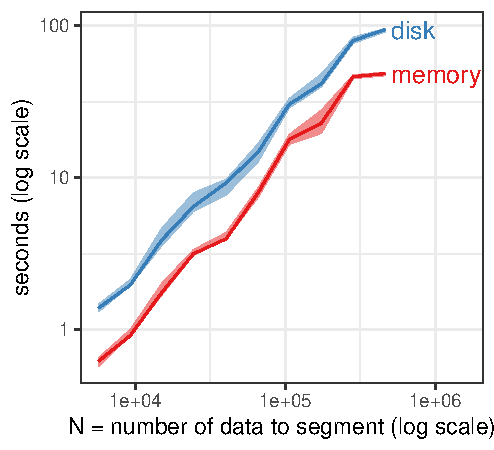
\includegraphics[width=0.5\textwidth]{jss-figure-disk-memory-compare-speed}

  \begin{itemize}
  \item Disk storage is only a constant factor slower than memory!
  \item Both are $O(N\log N)$ time.
  \item Memory implementation: $O(N \log N)$ memory! (too big)
  \item Disk implementation: $O(\log N)$ memory ($<1$GB), $O(N\log N)$
    disk.
  \end{itemize}

\end{frame}

\begin{frame}[fragile]
  \frametitle{Time/space to solve one penalty is $O(N \log N)$}

  Total time/space = $O(NI)$ where $I$ is the number of intervals
  (candidate changepoints) stored in every optimal cost function
  $\overline C_t(\mu)$.

  \begin{minipage}{0.48\textwidth}
    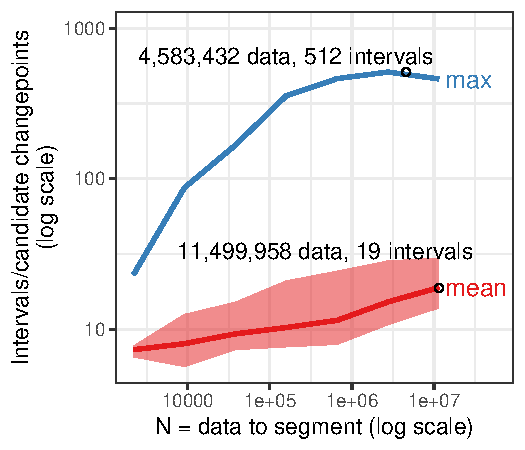
\includegraphics[width=\textwidth]{jss-figure-target-intervals-models}
    $I=O(\log N)$ intervals.
  \end{minipage}
  \begin{minipage}{0.48\textwidth}
    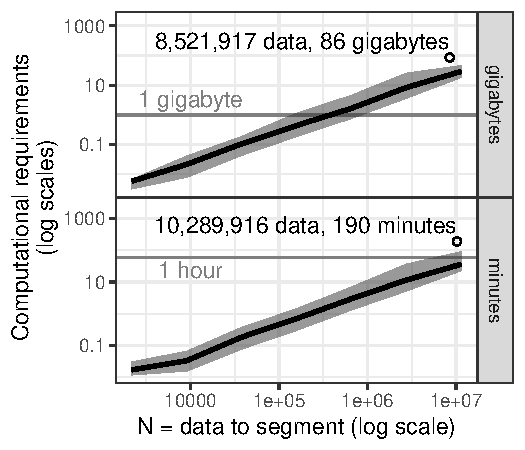
\includegraphics[width=\textwidth]{jss-figure-target-intervals-models-computation}
    Overall  $O(N \log N)$ complexity.
  \end{minipage}
  
\vskip 0.5cm
  But how to compute model with $O(\sqrt N)$ peaks?

\end{frame}

\begin{frame}
  \frametitle{Binary search algorithm using GFPOP to compute most
    likely model with at most $P^*$ peaks}
  \begin{algorithmic}[1]
  \STATE Input: data $\mathbf z\in\RR^N$, target peaks $P^*$.
  \STATE $\overline L,\overline p \gets \text{GFPOP}(\mathbf z, \lambda=0)$ // max peak model
  \STATE $\underline L,\underline p \gets \text{GFPOP}(\mathbf z, \lambda=\infty)$ // 0 peak model
  \STATE While $\underline p\neq P^*$ and $\overline p\neq P^*$:
  \begin{ALC@g}
    \STATE $\lambda=(\overline L-\underline L)/(\underline p-\overline p)$
    \STATE $L_{\text{new}},p_{\text{new}}\gets\text{GFPOP}(\mathbf z, \lambda)$
    \STATE If $p_{\text{new}}\in\{\underline p, \overline p\}$: return model with $\underline p$ peaks.
    \STATE If $p_{\text{new}} < P^*$: $\underline p\gets p_{\text{new}}$
    \STATE Else: $\overline p\gets p_{\text{new}}$
% > prob.i <- 3
% > fit.list$others[order(iteration)][, list(target.peaks=prob$peaks, iteration, under, over, penalty, peaks, total.cost)]
%    target.peaks iteration under over    penalty peaks total.cost
% 1:           33         1    NA   NA     0.0000  7487 -201361.96
% 2:           33         1    NA   NA        Inf     0  920923.98
% 3:           33         2     0 7487   149.8979   753  -24385.02
% 4:           33         3     0  753  1255.3904    47  153676.28
% 5:           33         4     0   47 16324.4191    10  310043.81
% 6:           33         5    10   47  4226.1495    21  214200.02
% 7:           33         6    21   47  2327.8360    33  177484.99
% > 
  \end{ALC@g}
  \STATE If $\underline p=P^*$: return model with $\underline p$ peaks.
  \STATE Else: return model with $\overline p$ peaks.
  \end{algorithmic}
\end{frame}

\begin{frame}
  \frametitle{Example run of binary search algorithm using GFPOP}
  One data set with $P^*=93$ peaks and $N=146,186$ data.
  \begin{tabular}{rrrrrr}
 iteration& $\underline p$& $\overline p$&    $\lambda$ & $p_{\text{new}}$& $L_{\text{new}}$\\
\hline
         1&    &    &     0& 68752&   -2570319\\
         1&    &    &        $\infty$&     0&   14239212\\
         2&     0& 68752&   244.4952&  4361&    1980119\\
         3&     0&  4361&  2811.0738&   188&    3676671\\
         4&     0&   188& 56183.7271&    55&    5330310\\
         5&    55&   188& 12433.3766&    98&    4108354\\
         6&    55&    98& 28417.5941&    72&    4584042\\
         7&    72&    98& 18295.6895&    83&    4336773\\
         8&    83&    98& 15227.9249&    90&    4218815\\
         9&    90&    98& 13807.6282&    95&    4146172\\
        10&    90&    95& 14528.5052&    92&    4188881\\
        11&    92&    95& 14236.0863&    94&    4160179\\
        12&    92&    94& 14350.6622&    93&    4174480
  \end{tabular}

  \alert{12 DP iterations much fewer than $93\times 2=186$ which would be
  required for Segment Neighborhood!}
\end{frame}


\begin{frame}
  \frametitle{Only $O(\log N)$ runs of GFPOP to compute $O(\sqrt N)$
    peaks}
  % Created by tikzDevice version 0.12.3.1 on 2021-08-27 11:08:28
% !TEX encoding = UTF-8 Unicode
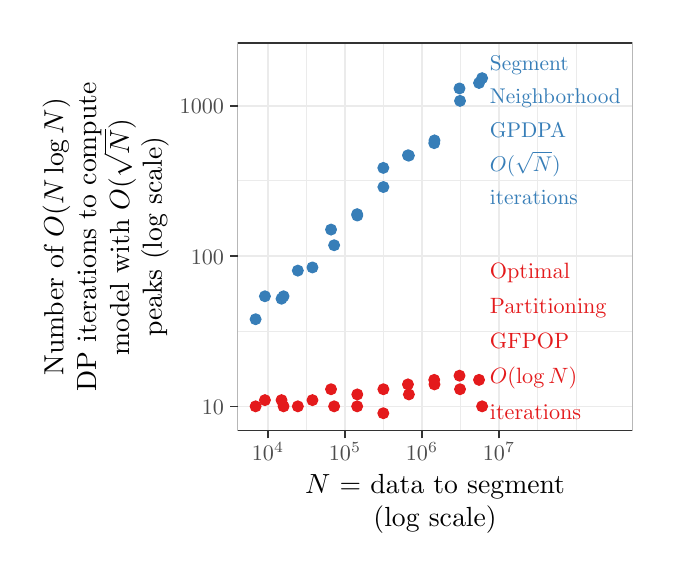
\begin{tikzpicture}[x=1pt,y=1pt]
\definecolor{fillColor}{RGB}{255,255,255}
\path[use as bounding box,fill=fillColor,fill opacity=0.00] (0,0) rectangle (224.04,187.90);
\begin{scope}
\path[clip] (  0.00,  0.00) rectangle (224.04,187.90);
\definecolor{drawColor}{RGB}{255,255,255}
\definecolor{fillColor}{RGB}{255,255,255}

\path[draw=drawColor,line width= 0.6pt,line join=round,line cap=round,fill=fillColor] (  0.00,  0.00) rectangle (224.04,187.90);
\end{scope}
\begin{scope}
\path[clip] ( 75.88, 42.21) rectangle (218.54,182.40);
\definecolor{fillColor}{RGB}{255,255,255}

\path[fill=fillColor] ( 75.88, 42.21) rectangle (218.54,182.40);
\definecolor{drawColor}{gray}{0.92}

\path[draw=drawColor,line width= 0.3pt,line join=round] ( 75.88, 78.22) --
	(218.54, 78.22);

\path[draw=drawColor,line width= 0.3pt,line join=round] ( 75.88,132.53) --
	(218.54,132.53);

\path[draw=drawColor,line width= 0.3pt,line join=round] (100.72, 42.21) --
	(100.72,182.40);

\path[draw=drawColor,line width= 0.3pt,line join=round] (128.56, 42.21) --
	(128.56,182.40);

\path[draw=drawColor,line width= 0.3pt,line join=round] (156.39, 42.21) --
	(156.39,182.40);

\path[draw=drawColor,line width= 0.3pt,line join=round] (184.22, 42.21) --
	(184.22,182.40);

\path[draw=drawColor,line width= 0.3pt,line join=round] (198.14, 42.21) --
	(198.14,182.40);

\path[draw=drawColor,line width= 0.6pt,line join=round] ( 75.88, 51.07) --
	(218.54, 51.07);

\path[draw=drawColor,line width= 0.6pt,line join=round] ( 75.88,105.37) --
	(218.54,105.37);

\path[draw=drawColor,line width= 0.6pt,line join=round] ( 75.88,159.68) --
	(218.54,159.68);

\path[draw=drawColor,line width= 0.6pt,line join=round] ( 86.81, 42.21) --
	( 86.81,182.40);

\path[draw=drawColor,line width= 0.6pt,line join=round] (114.64, 42.21) --
	(114.64,182.40);

\path[draw=drawColor,line width= 0.6pt,line join=round] (142.47, 42.21) --
	(142.47,182.40);

\path[draw=drawColor,line width= 0.6pt,line join=round] (170.30, 42.21) --
	(170.30,182.40);
\definecolor{drawColor}{RGB}{55,126,184}
\definecolor{fillColor}{RGB}{55,126,184}

\path[draw=drawColor,line width= 0.4pt,line join=round,line cap=round,fill=fillColor] ( 82.36, 82.55) circle (  1.96);

\path[draw=drawColor,line width= 0.4pt,line join=round,line cap=round,fill=fillColor] ( 85.73, 90.84) circle (  1.96);

\path[draw=drawColor,line width= 0.4pt,line join=round,line cap=round,fill=fillColor] ( 91.73, 89.95) circle (  1.96);

\path[draw=drawColor,line width= 0.4pt,line join=round,line cap=round,fill=fillColor] ( 92.46, 90.84) circle (  1.96);

\path[draw=drawColor,line width= 0.4pt,line join=round,line cap=round,fill=fillColor] ( 97.62,100.11) circle (  1.96);

\path[draw=drawColor,line width= 0.4pt,line join=round,line cap=round,fill=fillColor] (102.90,101.26) circle (  1.96);

\path[draw=drawColor,line width= 0.4pt,line join=round,line cap=round,fill=fillColor] (109.62,114.94) circle (  1.96);

\path[draw=drawColor,line width= 0.4pt,line join=round,line cap=round,fill=fillColor] (110.74,109.28) circle (  1.96);

\path[draw=drawColor,line width= 0.4pt,line join=round,line cap=round,fill=fillColor] (119.06,120.51) circle (  1.96);

\path[draw=drawColor,line width= 0.4pt,line join=round,line cap=round,fill=fillColor] (119.11,120.01) circle (  1.96);

\path[draw=drawColor,line width= 0.4pt,line join=round,line cap=round,fill=fillColor] (128.51,137.23) circle (  1.96);

\path[draw=drawColor,line width= 0.4pt,line join=round,line cap=round,fill=fillColor] (128.54,130.32) circle (  1.96);

\path[draw=drawColor,line width= 0.4pt,line join=round,line cap=round,fill=fillColor] (137.41,141.77) circle (  1.96);

\path[draw=drawColor,line width= 0.4pt,line join=round,line cap=round,fill=fillColor] (137.75,141.67) circle (  1.96);

\path[draw=drawColor,line width= 0.4pt,line join=round,line cap=round,fill=fillColor] (146.90,146.17) circle (  1.96);

\path[draw=drawColor,line width= 0.4pt,line join=round,line cap=round,fill=fillColor] (147.00,147.16) circle (  1.96);

\path[draw=drawColor,line width= 0.4pt,line join=round,line cap=round,fill=fillColor] (156.04,165.94) circle (  1.96);

\path[draw=drawColor,line width= 0.4pt,line join=round,line cap=round,fill=fillColor] (156.23,161.45) circle (  1.96);

\path[draw=drawColor,line width= 0.4pt,line join=round,line cap=round,fill=fillColor] (163.10,167.92) circle (  1.96);

\path[draw=drawColor,line width= 0.4pt,line join=round,line cap=round,fill=fillColor] (164.21,169.65) circle (  1.96);
\definecolor{drawColor}{RGB}{228,26,28}
\definecolor{fillColor}{RGB}{228,26,28}

\path[draw=drawColor,line width= 0.4pt,line join=round,line cap=round,fill=fillColor] ( 82.36, 51.07) circle (  1.96);

\path[draw=drawColor,line width= 0.4pt,line join=round,line cap=round,fill=fillColor] ( 85.73, 53.31) circle (  1.96);

\path[draw=drawColor,line width= 0.4pt,line join=round,line cap=round,fill=fillColor] ( 91.73, 53.31) circle (  1.96);

\path[draw=drawColor,line width= 0.4pt,line join=round,line cap=round,fill=fillColor] ( 92.46, 51.07) circle (  1.96);

\path[draw=drawColor,line width= 0.4pt,line join=round,line cap=round,fill=fillColor] ( 97.62, 51.07) circle (  1.96);

\path[draw=drawColor,line width= 0.4pt,line join=round,line cap=round,fill=fillColor] (102.90, 53.31) circle (  1.96);

\path[draw=drawColor,line width= 0.4pt,line join=round,line cap=round,fill=fillColor] (109.62, 57.25) circle (  1.96);

\path[draw=drawColor,line width= 0.4pt,line join=round,line cap=round,fill=fillColor] (110.74, 51.07) circle (  1.96);

\path[draw=drawColor,line width= 0.4pt,line join=round,line cap=round,fill=fillColor] (119.06, 51.07) circle (  1.96);

\path[draw=drawColor,line width= 0.4pt,line join=round,line cap=round,fill=fillColor] (119.11, 55.37) circle (  1.96);

\path[draw=drawColor,line width= 0.4pt,line join=round,line cap=round,fill=fillColor] (128.51, 48.58) circle (  1.96);

\path[draw=drawColor,line width= 0.4pt,line join=round,line cap=round,fill=fillColor] (128.54, 57.25) circle (  1.96);

\path[draw=drawColor,line width= 0.4pt,line join=round,line cap=round,fill=fillColor] (137.41, 59.00) circle (  1.96);

\path[draw=drawColor,line width= 0.4pt,line join=round,line cap=round,fill=fillColor] (137.75, 55.37) circle (  1.96);

\path[draw=drawColor,line width= 0.4pt,line join=round,line cap=round,fill=fillColor] (146.90, 60.63) circle (  1.96);

\path[draw=drawColor,line width= 0.4pt,line join=round,line cap=round,fill=fillColor] (147.00, 59.00) circle (  1.96);

\path[draw=drawColor,line width= 0.4pt,line join=round,line cap=round,fill=fillColor] (156.04, 62.15) circle (  1.96);

\path[draw=drawColor,line width= 0.4pt,line join=round,line cap=round,fill=fillColor] (156.23, 57.25) circle (  1.96);

\path[draw=drawColor,line width= 0.4pt,line join=round,line cap=round,fill=fillColor] (163.10, 60.63) circle (  1.96);

\path[draw=drawColor,line width= 0.4pt,line join=round,line cap=round,fill=fillColor] (164.21, 51.07) circle (  1.96);
\end{scope}
\begin{scope}
\path[clip] ( 75.88, 42.21) rectangle (218.54,182.40);
\definecolor{drawColor}{RGB}{228,26,28}

\node[text=drawColor,anchor=base west,inner sep=0pt, outer sep=0pt, scale=  0.80] at (167.05, 97.16) {Optimal};

\node[text=drawColor,anchor=base west,inner sep=0pt, outer sep=0pt, scale=  0.80] at (167.05, 84.49) {Partitioning};

\node[text=drawColor,anchor=base west,inner sep=0pt, outer sep=0pt, scale=  0.80] at (167.05, 71.82) {GFPOP};

\node[text=drawColor,anchor=base west,inner sep=0pt, outer sep=0pt, scale=  0.80] at (167.05, 59.15) {$O(\log N)$};

\node[text=drawColor,anchor=base west,inner sep=0pt, outer sep=0pt, scale=  0.80] at (167.05, 46.48) {iterations};
\definecolor{drawColor}{RGB}{55,126,184}

\node[text=drawColor,anchor=base west,inner sep=0pt, outer sep=0pt, scale=  0.77] at (167.05,172.47) {Segment};

\node[text=drawColor,anchor=base west,inner sep=0pt, outer sep=0pt, scale=  0.77] at (167.05,160.33) {Neighborhood};

\node[text=drawColor,anchor=base west,inner sep=0pt, outer sep=0pt, scale=  0.77] at (167.05,148.19) {GPDPA};

\node[text=drawColor,anchor=base west,inner sep=0pt, outer sep=0pt, scale=  0.77] at (167.05,136.06) {$O(\sqrt N)$};

\node[text=drawColor,anchor=base west,inner sep=0pt, outer sep=0pt, scale=  0.77] at (167.05,123.92) {iterations};
\definecolor{drawColor}{gray}{0.20}

\path[draw=drawColor,line width= 0.6pt,line join=round,line cap=round] ( 75.88, 42.21) rectangle (218.54,182.40);
\end{scope}
\begin{scope}
\path[clip] (  0.00,  0.00) rectangle (224.04,187.90);
\definecolor{drawColor}{gray}{0.30}

\node[text=drawColor,anchor=base east,inner sep=0pt, outer sep=0pt, scale=  0.80] at ( 70.93, 48.11) {10};

\node[text=drawColor,anchor=base east,inner sep=0pt, outer sep=0pt, scale=  0.80] at ( 70.93,102.42) {100};

\node[text=drawColor,anchor=base east,inner sep=0pt, outer sep=0pt, scale=  0.80] at ( 70.93,156.72) {1000};
\end{scope}
\begin{scope}
\path[clip] (  0.00,  0.00) rectangle (224.04,187.90);
\definecolor{drawColor}{gray}{0.20}

\path[draw=drawColor,line width= 0.6pt,line join=round] ( 73.13, 51.07) --
	( 75.88, 51.07);

\path[draw=drawColor,line width= 0.6pt,line join=round] ( 73.13,105.37) --
	( 75.88,105.37);

\path[draw=drawColor,line width= 0.6pt,line join=round] ( 73.13,159.68) --
	( 75.88,159.68);
\end{scope}
\begin{scope}
\path[clip] (  0.00,  0.00) rectangle (224.04,187.90);
\definecolor{drawColor}{gray}{0.20}

\path[draw=drawColor,line width= 0.6pt,line join=round] ( 86.81, 39.46) --
	( 86.81, 42.21);

\path[draw=drawColor,line width= 0.6pt,line join=round] (114.64, 39.46) --
	(114.64, 42.21);

\path[draw=drawColor,line width= 0.6pt,line join=round] (142.47, 39.46) --
	(142.47, 42.21);

\path[draw=drawColor,line width= 0.6pt,line join=round] (170.30, 39.46) --
	(170.30, 42.21);
\end{scope}
\begin{scope}
\path[clip] (  0.00,  0.00) rectangle (224.04,187.90);
\definecolor{drawColor}{gray}{0.30}

\node[text=drawColor,anchor=base,inner sep=0pt, outer sep=0pt, scale=  0.80] at ( 86.81, 31.34) {$10^4$};

\node[text=drawColor,anchor=base,inner sep=0pt, outer sep=0pt, scale=  0.80] at (114.64, 31.34) {$10^5$};

\node[text=drawColor,anchor=base,inner sep=0pt, outer sep=0pt, scale=  0.80] at (142.47, 31.34) {$10^6$};

\node[text=drawColor,anchor=base,inner sep=0pt, outer sep=0pt, scale=  0.80] at (170.30, 31.34) {$10^7$};
\end{scope}
\begin{scope}
\path[clip] (  0.00,  0.00) rectangle (224.04,187.90);
\definecolor{drawColor}{RGB}{0,0,0}

\node[text=drawColor,anchor=base,inner sep=0pt, outer sep=0pt, scale=  1.00] at (147.21, 19.50) {$N$ = data to segment};

\node[text=drawColor,anchor=base,inner sep=0pt, outer sep=0pt, scale=  1.00] at (147.21,  7.62) {(log scale)};
\end{scope}
\begin{scope}
\path[clip] (  0.00,  0.00) rectangle (224.04,187.90);
\definecolor{drawColor}{RGB}{0,0,0}

\node[text=drawColor,rotate= 90.00,anchor=base,inner sep=0pt, outer sep=0pt, scale=  1.00] at ( 12.89,112.30) {Number of $O(N \log N)$};

\node[text=drawColor,rotate= 90.00,anchor=base,inner sep=0pt, outer sep=0pt, scale=  1.00] at ( 24.77,112.30) {DP iterations to compute};

\node[text=drawColor,rotate= 90.00,anchor=base,inner sep=0pt, outer sep=0pt, scale=  1.00] at ( 36.65,112.30) {model with $O(\sqrt N)$};

\node[text=drawColor,rotate= 90.00,anchor=base,inner sep=0pt, outer sep=0pt, scale=  1.00] at ( 48.53,112.30) {peaks (log scale)};
\end{scope}
\end{tikzpicture}
 
  
\end{frame}

\begin{frame}
  \frametitle{Binary search only a log factor slower than solving one penalty}
  % Created by tikzDevice version 0.12.3 on 2020-01-08 13:36:11
% !TEX encoding = UTF-8 Unicode
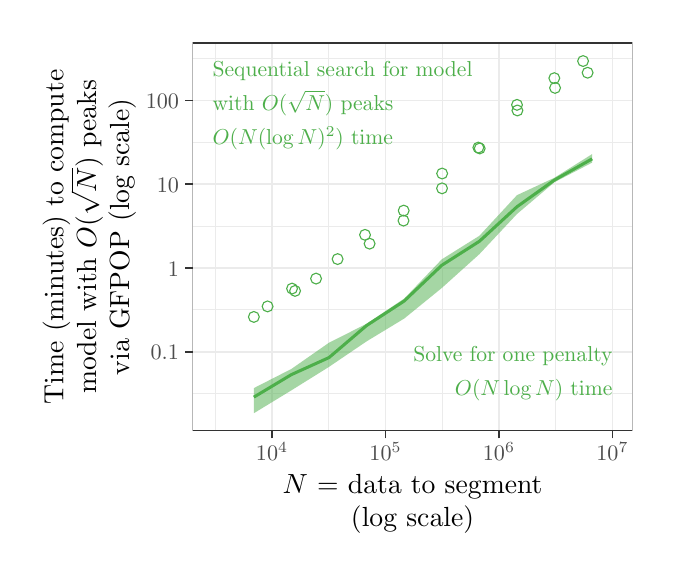
\begin{tikzpicture}[x=1pt,y=1pt]
\definecolor{fillColor}{RGB}{255,255,255}
\path[use as bounding box,fill=fillColor,fill opacity=0.00] (0,0) rectangle (224.04,187.90);
\begin{scope}
\path[clip] (  0.00,  0.00) rectangle (224.04,187.90);
\definecolor{drawColor}{RGB}{255,255,255}
\definecolor{fillColor}{RGB}{255,255,255}

\path[draw=drawColor,line width= 0.6pt,line join=round,line cap=round,fill=fillColor] (  0.00,  0.00) rectangle (224.04,187.90);
\end{scope}
\begin{scope}
\path[clip] ( 59.62, 42.21) rectangle (218.54,182.40);
\definecolor{fillColor}{RGB}{255,255,255}

\path[fill=fillColor] ( 59.62, 42.21) rectangle (218.54,182.40);
\definecolor{drawColor}{gray}{0.92}

\path[draw=drawColor,line width= 0.3pt,line join=round] ( 59.62, 55.66) --
	(218.54, 55.66);

\path[draw=drawColor,line width= 0.3pt,line join=round] ( 59.62, 85.93) --
	(218.54, 85.93);

\path[draw=drawColor,line width= 0.3pt,line join=round] ( 59.62,116.19) --
	(218.54,116.19);

\path[draw=drawColor,line width= 0.3pt,line join=round] ( 59.62,146.46) --
	(218.54,146.46);

\path[draw=drawColor,line width= 0.3pt,line join=round] ( 59.62,176.72) --
	(218.54,176.72);

\path[draw=drawColor,line width= 0.3pt,line join=round] ( 67.78, 42.21) --
	( 67.78,182.40);

\path[draw=drawColor,line width= 0.3pt,line join=round] (108.79, 42.21) --
	(108.79,182.40);

\path[draw=drawColor,line width= 0.3pt,line join=round] (149.80, 42.21) --
	(149.80,182.40);

\path[draw=drawColor,line width= 0.3pt,line join=round] (190.81, 42.21) --
	(190.81,182.40);

\path[draw=drawColor,line width= 0.6pt,line join=round] ( 59.62, 70.79) --
	(218.54, 70.79);

\path[draw=drawColor,line width= 0.6pt,line join=round] ( 59.62,101.06) --
	(218.54,101.06);

\path[draw=drawColor,line width= 0.6pt,line join=round] ( 59.62,131.32) --
	(218.54,131.32);

\path[draw=drawColor,line width= 0.6pt,line join=round] ( 59.62,161.59) --
	(218.54,161.59);

\path[draw=drawColor,line width= 0.6pt,line join=round] ( 88.28, 42.21) --
	( 88.28,182.40);

\path[draw=drawColor,line width= 0.6pt,line join=round] (129.29, 42.21) --
	(129.29,182.40);

\path[draw=drawColor,line width= 0.6pt,line join=round] (170.30, 42.21) --
	(170.30,182.40);

\path[draw=drawColor,line width= 0.6pt,line join=round] (211.31, 42.21) --
	(211.31,182.40);
\definecolor{drawColor}{RGB}{77,175,74}

\node[text=drawColor,anchor=base west,inner sep=0pt, outer sep=0pt, scale=  0.78] at ( 66.84,170.29) {Sequential search for model};

\node[text=drawColor,anchor=base west,inner sep=0pt, outer sep=0pt, scale=  0.78] at ( 66.84,158.00) {with $O(\sqrt N)$ peaks};

\node[text=drawColor,anchor=base west,inner sep=0pt, outer sep=0pt, scale=  0.78] at ( 66.84,145.71) {$O(N(\log N)^2)$ time};

\node[text=drawColor,anchor=base east,inner sep=0pt, outer sep=0pt, scale=  0.78] at (211.31, 67.26) {Solve for one penalty};

\node[text=drawColor,anchor=base east,inner sep=0pt, outer sep=0pt, scale=  0.78] at (211.31, 54.97) {$O(N \log N)$ time};
\definecolor{fillColor}{RGB}{77,175,74}

\path[fill=fillColor,fill opacity=0.50] ( 81.73, 57.66) --
	( 95.31, 64.59) --
	(108.89, 74.06) --
	(122.47, 80.91) --
	(136.06, 90.01) --
	(149.64,104.19) --
	(163.22,112.69) --
	(176.80,127.37) --
	(190.38,133.69) --
	(203.97,142.22) --
	(203.97,139.13) --
	(190.38,132.07) --
	(176.80,120.56) --
	(163.22,106.05) --
	(149.64, 93.83) --
	(136.06, 82.79) --
	(122.47, 74.55) --
	(108.89, 65.34) --
	( 95.31, 56.86) --
	( 81.73, 48.58) --
	cycle;

\path[draw=drawColor,line width= 1.1pt,line join=round] ( 81.73, 54.40) --
	( 95.31, 62.54) --
	(108.89, 68.69) --
	(122.47, 80.27) --
	(136.06, 89.12) --
	(149.64,102.04) --
	(163.22,110.70) --
	(176.80,123.18) --
	(190.38,132.86) --
	(203.97,140.50);

\path[draw=drawColor,line width= 0.4pt,line join=round,line cap=round] ( 81.73, 83.38) circle (  1.96);

\path[draw=drawColor,line width= 0.4pt,line join=round,line cap=round] ( 86.69, 87.18) circle (  1.96);

\path[draw=drawColor,line width= 0.4pt,line join=round,line cap=round] ( 95.53, 93.62) circle (  1.96);

\path[draw=drawColor,line width= 0.4pt,line join=round,line cap=round] ( 96.62, 92.78) circle (  1.96);

\path[draw=drawColor,line width= 0.4pt,line join=round,line cap=round] (104.21, 97.23) circle (  1.96);

\path[draw=drawColor,line width= 0.4pt,line join=round,line cap=round] (111.99,104.28) circle (  1.96);

\path[draw=drawColor,line width= 0.4pt,line join=round,line cap=round] (121.90,113.04) circle (  1.96);

\path[draw=drawColor,line width= 0.4pt,line join=round,line cap=round] (123.55,109.85) circle (  1.96);

\path[draw=drawColor,line width= 0.4pt,line join=round,line cap=round] (135.80,118.18) circle (  1.96);

\path[draw=drawColor,line width= 0.4pt,line join=round,line cap=round] (135.87,121.80) circle (  1.96);

\path[draw=drawColor,line width= 0.4pt,line join=round,line cap=round] (149.73,129.84) circle (  1.96);

\path[draw=drawColor,line width= 0.4pt,line join=round,line cap=round] (149.77,135.20) circle (  1.96);

\path[draw=drawColor,line width= 0.4pt,line join=round,line cap=round] (162.85,144.58) circle (  1.96);

\path[draw=drawColor,line width= 0.4pt,line join=round,line cap=round] (163.34,144.25) circle (  1.96);

\path[draw=drawColor,line width= 0.4pt,line join=round,line cap=round] (176.82,160.01) circle (  1.96);

\path[draw=drawColor,line width= 0.4pt,line join=round,line cap=round] (176.97,157.98) circle (  1.96);

\path[draw=drawColor,line width= 0.4pt,line join=round,line cap=round] (190.30,169.66) circle (  1.96);

\path[draw=drawColor,line width= 0.4pt,line join=round,line cap=round] (190.57,166.13) circle (  1.96);

\path[draw=drawColor,line width= 0.4pt,line join=round,line cap=round] (200.69,175.84) circle (  1.96);

\path[draw=drawColor,line width= 0.4pt,line join=round,line cap=round] (202.33,171.62) circle (  1.96);
\definecolor{drawColor}{gray}{0.20}

\path[draw=drawColor,line width= 0.6pt,line join=round,line cap=round] ( 59.62, 42.21) rectangle (218.54,182.40);
\end{scope}
\begin{scope}
\path[clip] (  0.00,  0.00) rectangle (224.04,187.90);
\definecolor{drawColor}{gray}{0.30}

\node[text=drawColor,anchor=base east,inner sep=0pt, outer sep=0pt, scale=  0.80] at ( 54.67, 67.84) {0.1};

\node[text=drawColor,anchor=base east,inner sep=0pt, outer sep=0pt, scale=  0.80] at ( 54.67, 98.10) {1};

\node[text=drawColor,anchor=base east,inner sep=0pt, outer sep=0pt, scale=  0.80] at ( 54.67,128.37) {10};

\node[text=drawColor,anchor=base east,inner sep=0pt, outer sep=0pt, scale=  0.80] at ( 54.67,158.63) {100};
\end{scope}
\begin{scope}
\path[clip] (  0.00,  0.00) rectangle (224.04,187.90);
\definecolor{drawColor}{gray}{0.20}

\path[draw=drawColor,line width= 0.6pt,line join=round] ( 56.87, 70.79) --
	( 59.62, 70.79);

\path[draw=drawColor,line width= 0.6pt,line join=round] ( 56.87,101.06) --
	( 59.62,101.06);

\path[draw=drawColor,line width= 0.6pt,line join=round] ( 56.87,131.32) --
	( 59.62,131.32);

\path[draw=drawColor,line width= 0.6pt,line join=round] ( 56.87,161.59) --
	( 59.62,161.59);
\end{scope}
\begin{scope}
\path[clip] (  0.00,  0.00) rectangle (224.04,187.90);
\definecolor{drawColor}{gray}{0.20}

\path[draw=drawColor,line width= 0.6pt,line join=round] ( 88.28, 39.46) --
	( 88.28, 42.21);

\path[draw=drawColor,line width= 0.6pt,line join=round] (129.29, 39.46) --
	(129.29, 42.21);

\path[draw=drawColor,line width= 0.6pt,line join=round] (170.30, 39.46) --
	(170.30, 42.21);

\path[draw=drawColor,line width= 0.6pt,line join=round] (211.31, 39.46) --
	(211.31, 42.21);
\end{scope}
\begin{scope}
\path[clip] (  0.00,  0.00) rectangle (224.04,187.90);
\definecolor{drawColor}{gray}{0.30}

\node[text=drawColor,anchor=base,inner sep=0pt, outer sep=0pt, scale=  0.80] at ( 88.28, 31.34) {$10^4$};

\node[text=drawColor,anchor=base,inner sep=0pt, outer sep=0pt, scale=  0.80] at (129.29, 31.34) {$10^5$};

\node[text=drawColor,anchor=base,inner sep=0pt, outer sep=0pt, scale=  0.80] at (170.30, 31.34) {$10^6$};

\node[text=drawColor,anchor=base,inner sep=0pt, outer sep=0pt, scale=  0.80] at (211.31, 31.34) {$10^7$};
\end{scope}
\begin{scope}
\path[clip] (  0.00,  0.00) rectangle (224.04,187.90);
\definecolor{drawColor}{RGB}{0,0,0}

\node[text=drawColor,anchor=base,inner sep=0pt, outer sep=0pt, scale=  1.00] at (139.08, 19.50) {$N$ = data to segment};

\node[text=drawColor,anchor=base,inner sep=0pt, outer sep=0pt, scale=  1.00] at (139.08,  7.62) {(log scale)};
\end{scope}
\begin{scope}
\path[clip] (  0.00,  0.00) rectangle (224.04,187.90);
\definecolor{drawColor}{RGB}{0,0,0}

\node[text=drawColor,rotate= 90.00,anchor=base,inner sep=0pt, outer sep=0pt, scale=  1.00] at ( 12.89,112.30) {Time (minutes) to compute};

\node[text=drawColor,rotate= 90.00,anchor=base,inner sep=0pt, outer sep=0pt, scale=  1.00] at ( 24.77,112.30) {     model with $O(\sqrt N)$ peaks};

\node[text=drawColor,rotate= 90.00,anchor=base,inner sep=0pt, outer sep=0pt, scale=  1.00] at ( 36.65,112.30) {     via GFPOP (log scale)};
\end{scope}
\end{tikzpicture}
 

  For $N=10^7$ only several hours of computation! (compare with weeks
  for Segment Neighborhood algorithm)
  
\end{frame}

\begin{frame}[fragile]
  \frametitle{Conclusions}

  \begin{itemize}
  \item Previous GPDPA was $O(N\sqrt N\log N)$ -- much too complex to
    compute a zero-error model with $O(\sqrt N)$ peaks for $N=10^7$
    data.
  \item Proposed GFPOP with binary search is $O(N(\log N)^2)$ time,
    $O(\log N)$ memory, $O(N\log N)$ disk -- optimal models are now
    possible to compute for large data.
  \item C++ code with R interface:
    \verb|PeakSegPipeline::PeakSegFPOP_disk|
    \url{https://github.com/tdhock/PeakSegPipeline}
  \item Future work: changepoint detection in large ecological data?
  \item Contact me: toby.hocking@nau.edu
  \item Thanks!
  \end{itemize}
  
\end{frame}

\begin{frame}
  \frametitle{For some data
 the desired number of peaks does not exist!}

One data set with $P^*=75$ and $N=66,031$ data.

\begin{tabular}{rrrrrr}
\small
 iteration& $\underline p$& $\overline p$&    $\lambda$ & $p_{\text{new}}$& $L_{\text{new}}$\\
  \hline
    1 &  &  & 0 & 29681 & -1495863.85 \\ 
    1 &  &  & $\infty$ &   0 & 1200631.42 \\ 
    2 &   0 & 29681 & 90.85 & 3445 & -1245181.37 \\ 
    3 &   0 & 3445 & 709.96 & 401 & -446632.57 \\ 
    4 &   0 & 401 & 4107.89 &  51 & 3105.03 \\ 
    5 &  51 & 401 & 1284.96 & 168 & -230152.31 \\ 
    6 &  51 & 168 & 1993.65 &  97 & -120725.83 \\ 
    7 &  51 &  97 & 2691.98 &  68 & -53946.18 \\ 
    8 &  68 &  97 & 2302.75 &  81 & -86423.80 \\ 
    9 &  68 &  81 & 2498.28 &  77 & -76891.10 \\ 
   10 &  68 &  77 & 2549.44 &  71 & -61722.09 \\ 
   11 &  71 &  77 & 2528.17 &  74 & -69330.62 \\ 
   12 &  74 &  77 & 2520.16 &  76 & -74374.78 \\ 
   13 &  \alert{74} &  \alert{76} & \alert{2522.08} &  \alert{76} & -74374.78 \\ 
\end{tabular}

\alert{No model exists between $\underline p=74$ and
  $\overline p=76$, so algo stops and returns the simpler model with 74 peaks.}

\end{frame}


\end{document}
